\documentclass[a4paper]{jpconf}
\usepackage{graphicx}


\usepackage{slashed}
\usepackage{subfigure}
%\usepackage{rotating}
\usepackage{multirow}
\usepackage{amsmath}
%\usepackage{units}
\setkeys{Gin}{width=\linewidth,totalheight=\textheight,keepaspectratio}
\graphicspath{{fig/}}

%
% My Macros
%
\usepackage{graphicx}
%\usepackage{drftcite}
\usepackage{pstricks}
\usepackage[figuresright]{rotating}
%
%
% Macro declarations
%
%---- SLASH
\def\slasha#1{#1\hskip-0.65em /}  %slasha per caratteri piccoli
\def\slashb#1{#1\hskip-1.3em /}   %slashb per quelli grandi
\def\slashc#1{#1\hskip-.4em /}
%
%---- UNITA` DI MISURA
\def \pb        {{\rm \, pb}}
\def \fb        {{\rm \, fb}}
\def \ipb       {{\rm \, pb^{-1}}}
\def \ifb       {{\rm \, fb^{-1}}}
\def \eV        {{\rm \,  eV}}
\def \keV       {{\rm \, keV}}
\def \MeV       {{\rm \, MeV}}
\def \GeV       {{\rm \, GeV}}
\def \TeV       {{\rm \, TeV}}
\def \TeVc      {\TeV/c}
\def \TeVcc     {\TeV/c^2}
\def \GeVc      {\GeV/c}
\def \GeVcc     {\GeV/c^2}
\def \MeVc      {\MeV/c}
\def \MeVcc     {\MeV/c^2}
%
%---- SIMBOLI
\def\ga{\mathrel{\raise.3ex\hbox{$>$\kern-.75em\lower1ex\hbox{$\sim$}}}}
\def\la{\mathrel{\raise.3ex\hbox{$<$\kern-.75em\lower1ex\hbox{$\sim$}}}}
\newcommand {\lesssim}
     {\,\raisebox{-0.6ex}{$\stackrel{\textstyle<}{\textstyle\sim}$}\,}
\newcommand {\gtrsim}
     {\,\raisebox{-0.6ex}{$\stackrel{\textstyle>}{\textstyle\sim}$}\,}
\newcommand{\ckm}{$\checkmark$}
%
%---- MISCELLANEA
%\newcommand {\slashed}[1] { \mbox{\rlap{\hbox{/}} #1 }}
\newcommand {\onehalf}    {\raisebox{0.1ex}{${\frac{1}{2}}$}}
\newcommand {\fivethirds} {\raisebox{0.1ex}{${\frac{5}{3}}$}}
\newcommand {\OR}         {{\tt OR}\,}
\newcommand {\BR}         {{\rm BR}\,}
\newcommand {\rts}        {\sqrt{s}}
\newcommand {\lumi}       {\mathcal{L}}
\newcommand {\Lumi}       {\int\lumi\mathrm{d}t}
\newcommand {\gradi}    {^\circ}
\newcommand {\de}         {\partial}
\newcommand {\um}         {\, \mu \rm m}
\newcommand {\nm}         {\rm \, nm}
\newcommand {\us}         {\, \mu \rm s}
\newcommand {\cm}         {\rm \, cm}
\newcommand {\mm}         {\rm \, mm}
\newcommand {\m}          {\rm \, m}
\newcommand {\km}         {\rm \, km}
\newcommand {\V}          {\rm \, V}
\newcommand {\T}          {\rm \, T}
\newcommand {\kV}         {\rm \, kV}
\newcommand {\kVm}        {\rm \, kV\! / \! m} 
\newcommand {\MVm}        {\rm \, MV\! / \! m} 
\newcommand {\ns}         {\rm \, ns} 
\newcommand {\ps}         {\rm \, ps} 
%
%---- THEORY groups & AOB
\newcommand {\gws}        {\mathrm{SU(2)_L \otimes U(1)_Y}}
\newcommand {\sul}        {\mathrm{SU(2)_L}}
\newcommand {\suc}        {\mathrm{SU(3)_C}}
\newcommand {\ul}         {\mathrm{U(1)_Y}}
\newcommand {\uem}        {\mathrm{U(1)_{em}}}
\newcommand {\sigmabar}   {\overline{\sigma}}
\newcommand {\gmunu}      {g^{\mu \nu}}
\newcommand {\munu}       {{\mu \nu}}
\newcommand {\obra}       {\langle 0 |}
\newcommand {\oket}       {| 0 \rangle}
%
%---- THEORY lepton fields
\newcommand {\LL}         {L^{\alpha}_{\mathrm L}}
\newcommand {\LLd}        {L^{\dagger \alpha}_{\mathrm L}}
\newcommand {\lL}         {\ell^{\alpha}_{\mathrm L}}
\newcommand {\lLd}        {\ell^{\dagger \alpha}_{\mathrm L}}
\newcommand {\ld}         {\ell^{\dagger \alpha}}
\newcommand {\lb}         {\overline{\ell}^{\alpha}}
\newcommand {\lR}         {\ell^{\alpha}_{\mathrm R}}
\newcommand {\lRd}        {\ell^{\dagger \alpha}_{\mathrm R}}
\newcommand {\nuL}        {\nu^{\alpha}_{\mathrm L}}
\newcommand {\nuLb}       {\overline{\nu}^{\alpha}_{\mathrm L}}
\newcommand {\nub}        {\overline{\nu}^{\alpha}}
\newcommand {\lept}       {\ell^\alpha}
\newcommand {\neut}       {\nu^{\alpha}}
\newcommand {\nuLd}       {\nu^{\dagger \alpha}_{\mathrm L}}
\newcommand {\Phid}       {\Phi^\dagger}
%
%---- THEORY quark fields
\newcommand {\up}         {u^{\alpha}}
\newcommand {\ub}         {\overline{u}^{\alpha}}
\newcommand {\down}       {d^{\alpha}}
\newcommand {\db}         {\overline{d}^{\alpha}}
\newcommand {\QL}         {Q^{\alpha}_{\mathrm L}}
\newcommand {\QLd}        {Q^{\dagger \alpha}_{\mathrm L}}
\newcommand {\UL}         {U^{\alpha}_{\mathrm L}}
\newcommand {\ULd}        {U^{\dagger \alpha}_{\mathrm L}}
\newcommand {\UR}         {U^{\alpha}_{\mathrm R}}
\newcommand {\URd}        {U^{\dagger \alpha}_{\mathrm R}}
\newcommand {\DL}         {D^{\alpha}_{\mathrm L}}
\newcommand {\DLd}        {D^{\dagger \alpha}_{\mathrm L}}
\newcommand {\DR}         {D^{\alpha}_{\mathrm R}}
\newcommand {\DRd}        {D^{\dagger \alpha}_{\mathrm R}}
\newcommand {\bfell}      {\ell\kern-0.4em
                           \ell\kern-0.4em
                           \ell\kern-0.4em
                           \ell }
\newcommand {\obfell}     {\overline{\ell}\kern-0.4em
                           \overline{\ell}\kern-0.4em
                           \overline{\ell}\kern-0.4em
                           \overline{\ell}}
\newcommand {\bfH}      {\, {\cal H}\kern-0.5em \kern-0.4em
                           {\cal H}\kern-0.5em \kern-0.4em
                           {\cal H}\kern0.1em }
\newcommand {\obfH}     {\, \overline{\cal H}\kern-0.5em \kern-0.4em 
                           \overline{\cal H}\kern-0.5em \kern-0.4em 
                           \overline{\cal H}\kern0.1em }
%
%---- PARTICELLE
\def \b             {{\mathrm b}}
\def \t             {{\mathrm t}}
\def \charm         {{\mathrm c}}
\def \d             {{\mathrm d}}
\def \u             {{\mathrm u}}
\def \e             {{\mathrm e}}
\def \q             {{\mathrm q}}
\def \g             {{\mathrm g}}
\def \p             {{\mathrm p}}
\def \s             {{\mathrm s}}
\def \n             {{\mathrm n}}
\def \h             {{\mathrm h}}
\def \l             {\ell} 
\def \f             {{\mathrm f}} 
%\def \f             {{f}} 
\def \A             {{\mathrm A}}
\def \B             {{\mathrm B}}
\def \D             {{\mathrm D}}
\def \K             {{\mathrm K}}
\def \X             {{\mathrm X}}
\def \Y             {{\mathrm Y}}
\def \W             {{\mathrm W}}
\def \H             {{\mathrm H}}
\def \Z             {{\mathrm Z}}
\def \S             {{\mathrm S}}
\def \N             {{\mathrm N}}
\def \L             {{\mathrm L}}
\def \R             {{\mathrm R}}
\def \P             {{\mathrm P}}
\def \G             {{\mathrm G}}
%
%---- Higgs
\newcommand {\ho}         {{\h^0}}
\newcommand {\Ho}         {{\H^0}}
\newcommand {\Ao}         {{\A^0}}
\newcommand {\Hpm}        {{\H^\pm}}
\newcommand {\clsb}       {{\mathrm CL_{\rm s+b}}}
\newcommand {\clb}        {{\mathrm CL_{\rm b}}}
%
%---- SUSY
\newcommand {\dm}         {\Delta m}
\newcommand {\dM}         {\Delta M}
\newcommand {\ldm}        {\mbox{``low $\dm$''}}
\newcommand {\hdm}        {\mbox{``high $\dm$''}}
\newcommand {\nnc}        {{\overline{\mathrm N}_{95}}}
\newcommand {\snc}        {{\overline{\sigma}_{95}}}
\newcommand {\susy}       {{supersymmetry}}
\newcommand {\susyc}      {{supersymmetric}}
\newcommand {\aj}         {\mbox{\sf AJ}}
\newcommand {\ajl}        {\mbox{\sf AJL}}
\newcommand {\llh}        {\mbox{\sf LLH}}
%
%---- SPARTICELLE
\newcommand {\rpc}     {{\rm RPC}}
\newcommand {\rpv}     {{\rm RPV}}
\newcommand {\sfe}     {{\tilde{\f}}}
\newcommand {\sfL}     {{\tilde{\f}_{\mathrm L}}}
\newcommand {\sfR}     {{\tilde{\f}_{\mathrm R}}}
\newcommand {\sfone}   {{\tilde{\f}_{1}}}
\newcommand {\sftwo}   {{\tilde{\f}_{2}}}
\newcommand {\sneu}    {{\tilde{\nu}}}
\newcommand {\wino}    {{\mathrm{\widetilde{W}}}}
\newcommand {\bino}    {{\mathrm{\widetilde{B}}}}
\newcommand {\se}      {{\mathrm{\tilde{e}}}}
\newcommand {\seR}     {{\mathrm{\tilde{e}_{R}}}}
\newcommand {\seL}     {{\mathrm{\tilde{e}_{L}}}}
\newcommand {\st}      {{\mathrm{\tilde{\tau}}}}
\newcommand {\stR}     {{\mathrm{\tilde{\tau}_{R}}}}
\newcommand {\stL}     {{\mathrm{\tilde{\tau}_{L}}}}
\newcommand {\stone}   {{\mathrm{\tilde{\tau}_{1}}}}
\newcommand {\sttwo}   {{\mathrm{\tilde{\tau}_{2}}}}
\newcommand {\sm}      {{\mathrm{\tilde{\mu}}}}
\newcommand {\smR}     {{\mathrm{\tilde{\mu}_{R}}}}
\newcommand {\smL}     {{\mathrm{\tilde{\mu}_{L}}}}
\newcommand {\Sup}     {{\mathrm{\tilde{u}}}}
\newcommand {\suR}     {{\mathrm{\tilde{u}_{R}}}}
\newcommand {\suL}     {{\mathrm{\tilde{u}_{L}}}}
\newcommand {\sdo}     {{\mathrm{\tilde{d}}}}
\newcommand {\sdR}     {{\mathrm{\tilde{d}_{R}}}}
\newcommand {\sdL}     {{\mathrm{\tilde{d}_{L}}}}
\newcommand {\sch}     {{\mathrm{\tilde{c}}}}
\newcommand {\scR}     {{\mathrm{\tilde{c}_{R}}}}
\newcommand {\scL}     {{\mathrm{\tilde{c}_{L}}}}
\newcommand {\sst}     {{\mathrm{\tilde{s}}}}
\newcommand {\ssR}     {{\mathrm{\tilde{s}_{R}}}}
\newcommand {\ssL}     {{\mathrm{\tilde{s}_{L}}}}
\newcommand {\stopR}   {{\tilde{\mathrm{t}}_{R}}}
\newcommand {\stopL}   {{\tilde{\mathrm{t}}_{L}}}
\newcommand {\stopone} {{\tilde{\mathrm{t}}_{1}}}
\newcommand {\stoptwo} {{\mathrm{\tilde{t}_{2}}}}
\newcommand {\sto}     {{\tilde{\mathrm{t}}}}
\newcommand {\SQ}      {{\mathrm{\widetilde{Q}}}}
\newcommand {\STO}     {{\mathrm{\widetilde{T}}}}
\newcommand {\glu}     {{\mathrm{\tilde{g}}}}
\newcommand {\sbotR}   {{\mathrm{\tilde{b}_{R}}}}
\newcommand {\sbotL}   {{\mathrm{\tilde{b}_{L}}}}
\newcommand {\sbotone} {{\mathrm{\tilde{b}_{1}}}}
\newcommand {\sbottwo} {{\mathrm{\tilde{b}_{2}}}}
\newcommand {\sbot}    {{\tilde{\mathrm{b}}}}
\newcommand {\squa}    {{\tilde{\mathrm{q}}}}
\newcommand {\squal}   {{\tilde{\mathrm{q}}_{\rm L}}}
\newcommand {\squar}   {{\tilde{\mathrm{q}}_{\rm R}}}
\newcommand {\sqL}     {{\tilde{\mathrm{q}}_{\rm L}}}
\newcommand {\sqR}     {{\tilde{\mathrm{q}}_{\rm R}}}
\newcommand {\snu}     {{\tilde{\nu}}}
\newcommand {\snue}    {{\tilde{\nu}_{\mathrm e}}}
\newcommand {\snum}    {{\tilde{\nu}_{\mu}}}
\newcommand {\snut}    {{\tilde{\nu}_{\tau}}}
\newcommand {\neu}     {{\chi}}
\newcommand {\chap}    {{\chi^+}}
\newcommand {\cham}    {{\chi^-}}
\newcommand {\chapm}   {{\chi^\pm}}

%
%---- SUSY PARAMETRI
\newcommand {\thstop} {\mathrm{\theta_{\tilde{t}}}}
\newcommand {\thsbot} {\mathrm{\theta_{\tilde{b}}}}
\newcommand {\thsqua} {\mathrm{\theta_{\tilde{q}}}}
\newcommand {\Mcha}{M_{\chi^\pm}}
\newcommand {\Mchi}{M_\chi}
\newcommand {\Msnu}{M_{\tilde{\nu}}}
\newcommand {\tanb}{\tan\beta}
%
%---- ABBREVIAZIONI

%
%---- PROCESSI FISICI
\newcommand {\rb}    {{\rm R_{\b}}}
\newcommand {\qq}    {{\q \overline{\q}}}
\newcommand {\bb}    {{\b \overline{\b}}}
\newcommand {\cc}    {{\charm \overline{\charm}}}
\newcommand {\ff}    {{\f \overline{\f}}}
\newcommand {\el}    {{\e ^+}}
\newcommand {\po}    {{\e ^-}}
\newcommand {\ee}    {{\e ^+ \e ^-}}
\newcommand {\fbody} {{\sto \to \b \chi {\rm f \bar{f}'}}}
\newcommand {\gaga}  {\gamma\gamma}
\newcommand {\ggqq}  {\gamma\gamma \rightarrow \q\overline{\q}}
\newcommand {\ggtt}  {\gamma\gamma \rightarrow \tau^{+}\tau^{-}}
\newcommand {\qqg}   {\q\overline{\q}\gamma}
\newcommand {\ttg}   {\tau^{+}\tau^{-}\gamma}
\newcommand {\wenu}  {{\rm We\nu_\e}}
\newcommand {\gsZ}   {\gamma^\star\mathrm{Z}}
\newcommand {\ggh}   {\gamma\gamma\rightarrow{\mathrm{hadrons}}}
\newcommand {\ZZg}   {\mathrm ZZ^{*}/\gamma^{*}}
\newcommand {\ZZ}    {{\mathrm ZZ}}
%
%---- VARIABILI
\newcommand {\zo}      {{z_0}}
\newcommand {\ip}      {{d_0}}
%\newcommand {\thr}     {{T_{\rm thrust}}}
\newcommand {\thr}     {{{\rm thrust}}}
\newcommand {\athr}    {{\hat{\rm a}_{\rm thrust}}}
\newcommand {\ththr}   {{\theta_{\rm thrust}}}
\newcommand {\acol}    {{\Phi_{\rm acol}}}
\newcommand {\acop}    {{\Phi_{\rm acop}}}
\newcommand {\acopt}   {{\Phi_{\rm acop_T}}}
\newcommand {\thpoint} {\theta_{\rm point}}
\newcommand {\thscat}  {\theta_{\rm scat}}
\newcommand {\etwelve} {E_{12\gradi}}
\newcommand {\ethirty} {E_{30\gradi}}
\newcommand {\eiso}[1] {E^{\, \triangleleft 30\gradi}_{#1}}
\newcommand {\phimiss} {{\phi_{\vec{p}_{\rm miss}}}}
\newcommand {\ewedge}  {E(\phi_{\vec{p}_{\rm miss}}\pm 15\gradi)}
%\newcommand {\ewedge}  {{E_{\rm w}}}
\newcommand {\evis}    {E_{\rm vis}}
\newcommand {\etot}    {E_{\rm vis}}
\newcommand {\emis}    {E_{\rm miss}}
\newcommand {\mvis}    {M_{\rm vis}}
\newcommand {\mtot}    {M_{\rm vis}}
\newcommand {\mmis}    {M_{\rm miss}}
\newcommand {\mhad}    {M^{\rm ex \, \ell_1}_{\rm vis}}
\newcommand {\mhadtwo} {M^{\rm ex \, \ell_1\ell_2}_{\rm vis}}
\newcommand {\ehad}    {E^{\rm NH}_{\rm vis}}
\newcommand {\epho}    {E^{\gamma}_{\rm vis}}
\newcommand {\echa}    {E^{\rm ch}_{\rm vis}}
\newcommand {\nch}     {{N_{\rm ch}}}
\newcommand {\elept}   {E_{\rm lept}}
\newcommand {\elepone} {E_{\ell _1}}
\newcommand {\eleptwo} {E_{\ell _2}}
\newcommand {\pvis}    {{\vec{p}_{\rm vis}}}
\newcommand {\pmis}    {{\vec{p}_{\rm miss}}}
\newcommand {\thmiss}  {{\theta_{\pmis}}}
\newcommand {\pt}      {{p_{\rm t}}}
\newcommand {\ptch}    {{p_{\rm t}^{\rm ch}}}
\newcommand {\pch}    {{p^{\rm ch}}}
\newcommand {\pz}      {{p_z}}
\newcommand {\ptnoNH}  {{p_{\rm t}^{\rm ex \, NH}}}
\newcommand {\puds}    {{P_{\rm uds}}}
%
\newcommand {\pmiss}   {{P\!\!\!\,\!/ }}
\newcommand {\emiss}   {{E\!\!\!\,\!/ }}
%
%
% no more of Christian's random capitalization!
% more of mine
\newcommand{\brchal}{\cal{B}($\PCha \rightarrow \ell\nu\PChi\ $)}
\newcommand{\M}{M_{2}}
\newcommand{\Mp}{M_{2}}
\newcommand{\sigbg}{\sigma_{\mathrm{bg}}}
\newcommand{\ww}   {\mathrm {WW}}
\newcommand{\zz}   {\mathrm Z\gamma^{*}}
\newcommand{\ewnu} {\mathrm{eW}\nu}
\newcommand{\eez}  {\mathrm {eeZ}}
\newcommand{\gagall}{{\gamma\gamma\rightarrow \ell\ell }}
\newcommand{\Pstaup}{{\widetilde{\tau}_{1}}}
\newcommand{\Pstaul}{{\widetilde{\tau}_{L}}}
\newcommand{\Pstaur}{{\widetilde{\tau}_{R}}}
\newcommand{\mzero}{m_{0}}
\newcommand{\msnu}{M_{\tilde{\nu}}}
\newcommand{\mcha}{M_{\chi^{\pm}}}
\newcommand{\mchi}{M_{\chi}}
\newcommand{\mstau}{M_{{\widetilde{\tau}_{1}}}}
\newcommand{\atau}{A_{\tau}}
\newcommand{\chsnu}{\PCha \rightarrow \ell \tilde{\nu}}
\newcommand{\chstau}{\PCha \rightarrow \tilde{\tau}_{1}\nu}
\newcommand{\chlep}{\PCha \rightarrow \ell\nu\chi}
\newcommand{\Tcsq}{\mathrm{TeV}/c^2}
% new for thesis
\newcommand{\nobs}{N_{\mathrm{obs}}}
\newcommand{\nlim}{N_{\mathrm{lim}}}
\newcommand{\Brl}{\cal{B}_{\ell}}
\newcommand{\leff} {\mathcal{L}_{\mathrm{eff}}}
\newcommand{\dedx}{{\mathrm{d}}E/{\mathrm{d}}x}
\newcommand{\chtau}{\PCha \rightarrow \tau\nu\chi}
\newcommand{\ssqtw}{\sin^{2}\theta_{\mathrm W}}
%\newcommand{\PSql}{\tilde{\mathrm q}_L}
%\newcommand{\PSqr}{\tilde{\mathrm q}_R}
%\newcommand{\PSq1}{\tilde{\mathrm q}_1}
%\newcommand{\PSq2}{\tilde{\mathrm q}_2}
%\newcommand{\ww}{{\mathrm WW}}
%\newcommand{\zz}{{\mathrm Z\gamma^{*}}}
%\newcommand{\eez}{{\mathrm eeZ}}
\newcommand{\nnz}{{\mathrm \nu\bar{\nu}Z}}
% added by bill
\def \ggll    {\gamma\gamma \rightarrow \ell^{+}{\ell}^{-}}
\def \tautau  {\mathrm \tau^{+}\tau^{-}}
\def \ffg  {f\bar{f}(\gamma)}
\def \lll   {\ell^{+}{\ell}^{-}}
\def \ww   {\mathrm WW}
\def \zz   {\mathrm Z\gamma^{*}}
\def \znn  {\mathrm Z\nu\nu}
\def \zee  {\mathrm Zee}
\def \rts  {\sqrt{s}}
\def \mstop {m_{\tilde{\mathrm{t}}}}
\def \msnu  {m_{\tilde{\nu}}}
\def \elow   {E_{12^{\circ}}}
\def \gev    { \, \mathrm{GeV}/\it{c}^{\mathrm{2}}}
\def \gvm    { \, \mathrm{GeV}/\it{c}}
\def \mx     {M_{\mathrm{eff}}} 
\newcommand{\neutr}{\chi}
%end fabio



%dalla mia pretesi

%\def \X             {\mathrm X} 
%\def \V             {\mathrm V} 
\def \Zcc           {\Z \to \charm \bar{\charm} }
\def \Zbb           {\Z \to \b \bar{\b} }
\def \decDS         {\D^{*+} \to \D^0 \pi^+}
\def \decsDS        {\D^{*+} \to \D^0 \pi^+_s}
\def \deckp         {\D^{0} \to \K^- \pi^+}
\def \deckppp       {\D^{0} \to \K^- \pi^+ \pi^+ \pi^-}
\def \deckpp        {\D^{0} \to \K^- \pi^+ \pi^0}
\def \deckpS        {\D^{0} \to \K^- \pi^+ (\pi^0)}
\def \decskp        {\D^{*+} \to \pi^{+}_{s} \K^- \pi^+}
\def \decskppp      {\D^{*+} \to \pi^{+}_{s} \K^- \pi^+ \pi^+ \pi^-}
\def \decskpp       {\D^{*+} \to \pi^{+}_{s} \K^- \pi^+ \pi^0}
\def \decskpS       {\D^{*+} \to \pi^{+}_{s} \K^- \pi^+ (\pi^0)}
\def \epsc          {\varepsilon_{\charm}}
\def \epsb          {\varepsilon_{\b}}
\def \pctod         {P_{\charm \to \D^*}}
\def \pbtod         {P_{\b \to \D^*}}
%\def \R             {{\mathrm R}}
\def \Gbb           {\Gamma_{\b\bar{\b}}}
\def \Gcc           {\Gamma_{\charm\bar{\charm}}}
\def \Gh            {\Gamma_{\mathrm h}}
%
% End of my macros
%

\def\centeron#1#2{{\setbox0=\hbox{#1}\setbox1=\hbox{#2}\ifdim
\wd1>\wd0\kern.5\wd1\kern-.5\wd0\fi
\copy0\kern-.5\wd0\kern-.5\wd1\copy1\ifdim\wd0>\wd1
\kern.5\wd0\kern-.5\wd1\fi}}
\def\ltap{\;\centeron{\raise.35ex\hbox{$<$}}{\lower.65ex\hbox{$\sim$}}\;}
\def\gtap{\;\centeron{\raise.35ex\hbox{$>$}}{\lower.65ex\hbox{$\sim$}}\;}
\def\gsim{\mathrel{\gtap}}
\def\lsim{\mathrel{\ltap}}


% Definitions
\def \usedlumi {4.51\fbinv}
\def \chic {\chi_{c}}
\def \Chizero {\chi_{c0}}
\def \Chione {\chi_{c1}}
\def \Chitwo {\chi_{c2}}
\def \theratio {N_{\Chitwo}/N_{\Chione}}
\def \eoneetwo {{\varepsilon_{1}/\varepsilon_{2}}} 
\def \JPsi{\rm J/\psi}
\def \cPgg{\gamma}
\def \pt{$\p_{\rm T}$~}

% A useful Journal macro
\def\Journal#1#2#3#4{{#1} {\bf #2}, #3 (#4)}

\begin{document}
\title{An innovative seeding technique for photon conversion reconstruction at CMS}

\author{$^1$D~Giordano and $^2$G~Sguazzoni}

\address{$^1$CERN, Information Technology Department, Experiment Support Group, Geneva, Switzerland}
\address{$^2$INFN, Firenze, Italy}


\ead{domenico.giordano@cern.ch, giacomo.sguazzoni@cern.ch}

\begin{abstract}
The conversion of photons into electron-positron pairs in the detector material is a nuisance in the event reconstruction of high energy physics experiments, since the measurement of the electromagnetic component of interaction products results degraded. Nonetheless this unavoidable detector effect can be also extremely useful. The reconstruction of photon conversions can be used to probe the detector material and to accurately measure soft photons that come from radiative decays in heavy flavor physics. In fact a converted photon can be measured with very high momentum resolution by exploiting the excellent reconstruction of charged tracks of a tracking detector as the one of CMS at LHC. The main issue is that photon conversion tracks are difficult to reconstruct for standard reconstruction algorithms. They are typically soft and very displaced from primary interaction vertex. An innovative seeding technique that exploits the peculiar photon conversion topology, successfully applied in the CMS track reconstruction sequence, is presented. The performances of this technique and the substantial enhancement of photon conversion reconstruction efficiency are discussed. Application examples are given.
\end{abstract}


%\thispagestyle{empty}
\section{Introduction}
\label{introductions}

The precise and efficient determination of charged-particle momenta is a
critical component of the physics program of the LHC experiments, 
as it impacts the ability to
reconstruct leptons, charged hadrons and jets which
are the basic physics objects needed to study $pp$ collisions.
Achieving the necessary momentum resolution requires precise tracking in a high magnetic field. This has been obtained by  the two LHC general purpose experiments    adopting a design with the inner tracking systems in a solenoidal magnetic field.
%, followed by electromagnetic and hadronic calorimeters, and finally by muon detectors. 

What makes  track reconstruction difficult is  
the large number of hits in the tracking detectors
produced by the many tracks resulting from several $pp$ interactions in the same bunch crossing. In order to mitigate this issue the hit occupancy is kept low using highly granular sensors and, consequently, a high number of electronic channels (several millions) for their front-end readout at the cost of an increase of material in the tracking volume. These channels need to be powered, controlled, read-out through  complex systems of cables and optical fibers. Moreover they have to dissipate a considerable amount of heat, hence a capillary cooling system is also required.
The consequent amount of material  contained in the detectors and support structures, the associated electronics, and the power-supply and cooling services is not negligible and has effect on the tracking performance because of multiple scattering, energy loss and electron bremsstrahlung. 
For this reason the track reconstruction has to properly take into account the amount of material in the tracking volume: amount of material to be known with extreme accuracy.  
This material  affects also the overall event topology and its reconstruction because of photon conversions and nuclear interactions that modify the energy flow through the inner detector.

This unavoidable detector effect   can be also turned into an extremely useful tool. For instance the reconstruction of photon conversions can be used to probe the detector material and to accurately measure soft photons produced in radiative decays of heavy flavor particles. %In fact a converted photon can be measured with very high momentum resolution by exploiting the excellent reconstruction of charged tracks by the tracking detector. 
 
In this paper we will discuss the impact of the photon conversions in the event reconstruction at LHC.  We will refer to the CMS detector~\cite{JINST} , even if most of the concepts discussed can be applied also to other detectors. 
In the following sections a description of the CMS detector will be provided as well as some examples of the  problems and bonus due to the photon conversions inside the tracking volume.
We will summarize the current methods for the reconstruction of photon conversions and describe an innovative additional technique that allows to increase their reconstruction efficiency.


\section{The CMS detector}



The Compact Muon Solenoid (CMS) features an all-silicon tracker, a lead tungstate crystal electromagnetic calorimeter (ECAL), and a brass-scintillator hadronic calorimeter (HCAL), all contained inside a  $3.8\,{\rm T}$  superconducting solenoid.
The strong magnetic field  enables the measurement of charged
particle momenta over more than four orders of magnitude, from less than
$100\MeVc$ to more than $1\TeVc$, by reconstructing their trajectories as they
traverse the CMS inner tracking system.  
The iron return yoke of the solenoid is interspersed with gas detectors that are used to identify muons.


The CMS Tracker, shown
in~Fig.~\ref{fig:tklayout}, consists of 1\,440 silicon pixel and 15\,148 silicon strip detector modules, covering
the region from $4\cm$ to $110\cm$ in radius, and within $280\cm$ on either
side of the collision point along the LHC beam axis. The tracker
acceptance extends up to a pseudo-rapidity of $\left | \eta \right | < 2.5$.
The pseudo-rapidity $\eta$ is defined as $\rm  -log[tan(\theta/2)]$, where $\theta$ is the polar angle with respect to the direction of the LHC counter-clockwise beam, and $\phi$ is the azimuthal angle in the plane orthogonal to the beams.
The tracker detector  provides an impact parameter resolution of $\sim 15 \mu$m and a transverse momentum ($p_{\rm T}$) resolution of about 1.5\,\% for 100~GeV/$c$ particles.
The calorimeter towers are projective and finely segmented, with $\rm \Delta\phi \sim \Delta\eta \sim 0.087$ in the central region, allowing precise reconstruction of the $e/\gamma$ position and energy.  

\begin{figure}[h!]
  \begin{center}
    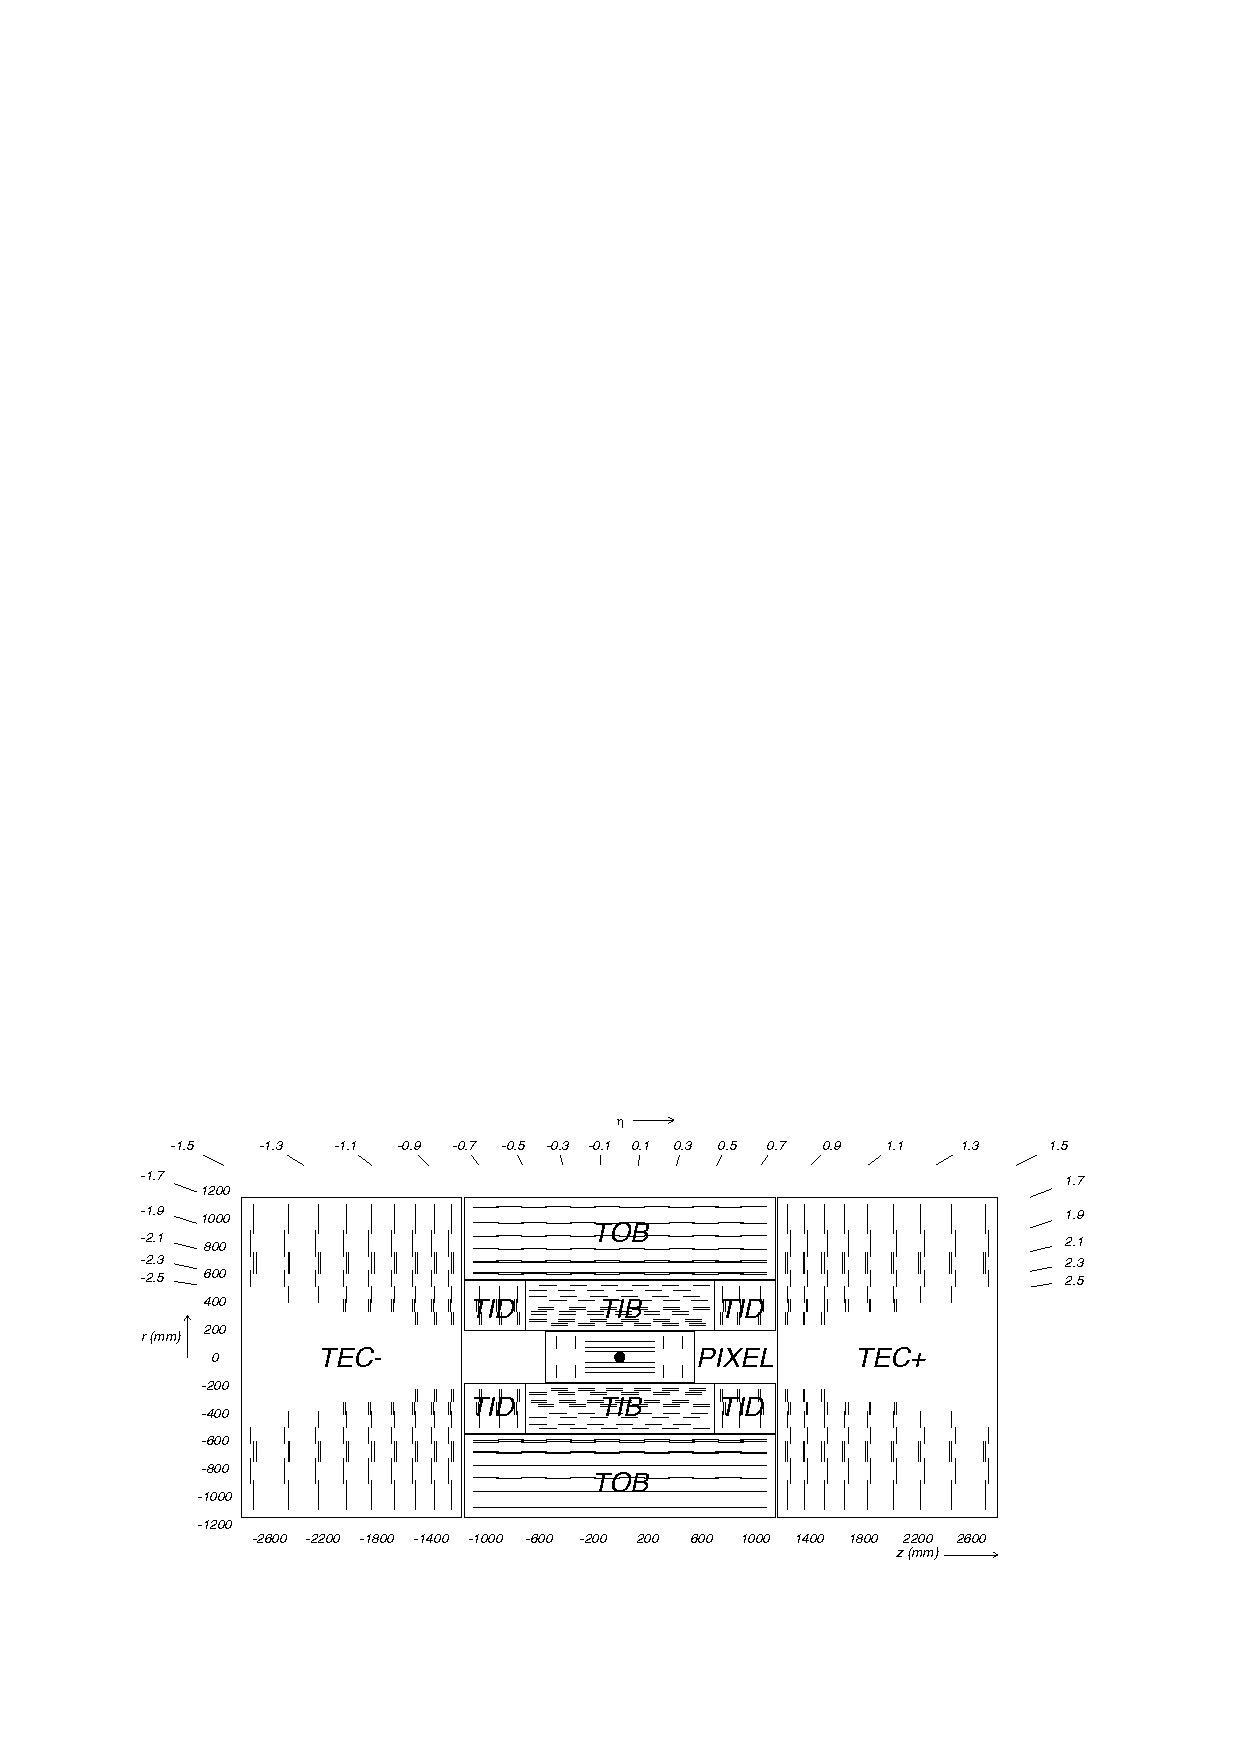
\includegraphics[width=0.8\textwidth]{fig/general_layout.pdf}
    \caption{Schematic cross section through the CMS tracker. Each line represents a detector module. Double lines indicate back-to-back modules which deliver stereo hits.}
    \label{fig:tklayout}
  \end{center}
\end{figure}

\begin{figure}[h!]
  \begin{center}
    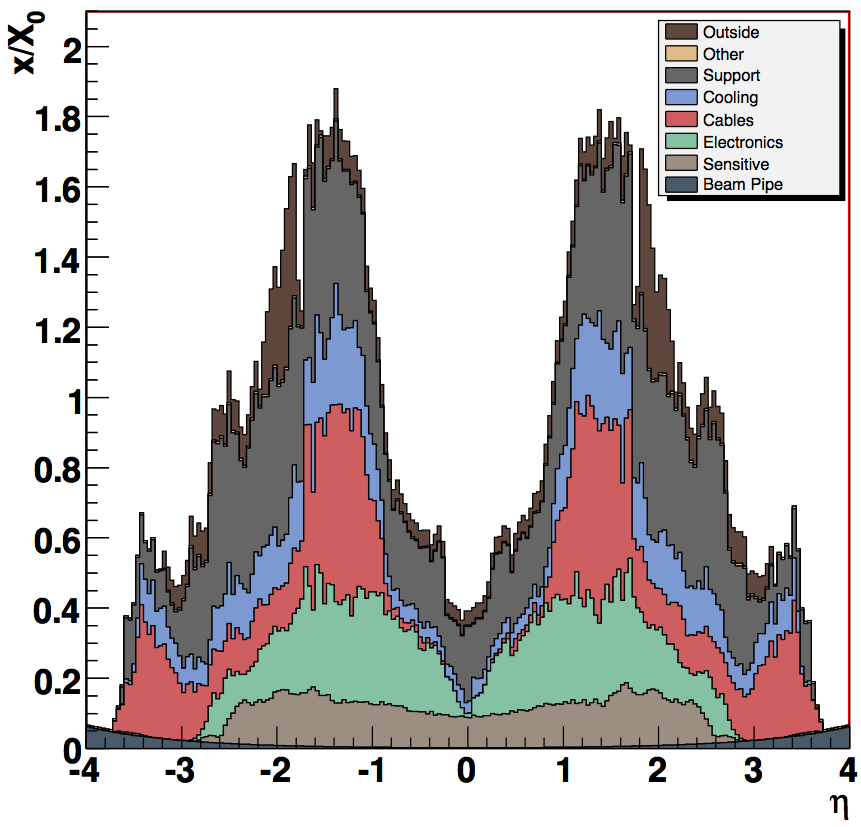
\includegraphics[width=0.4\textwidth]{fig/trackerMaterialbudget.png}
    \caption{Material budget inside the CMS Tracker volume in units of radiation length as a function of pseudorapidity $\eta$ broken down into the functional contributions.}
    \label{fig:tkmaterial}
  \end{center}
\end{figure}



Figure~\ref{fig:tkmaterial} shows the material budget of the CMS tracker in units of radiation length (X$_0$). 
The overall material crossed by a particle traversing the Tracker volume can exceed 1 X$_0$. 
It increases from 0.4~X$_0$ at $\eta \sim 0$ to about 1.8~X$_0$ at $|\eta| \sim 1.4$, beyond which it falls to about 1~X$_0$ at $|\eta| \sim 2.5$.
The largest contribution to the Tracker mass is by far represented by the passive structures having the largest uncertainty on their overall amount and can have a sensible impact on the expected physics performance. 



\section{Effects of the photon conversions}


As a consequence  of the amount of material shown in Fig.~\ref{fig:tkmaterial}, up to 70\% of photons traversing the CMS Tracker material converts into  $e^+ e^-$ pairs, resulting in a large fraction of secondary electrons. 
Most of these photons are from ${\rm \pi^0}  \to \gamma\gamma$ decays in jets. Other sources are prompt photons and the photon emitted by bremsstrahlung before an electron reaches the electromagnetic calorimeter. 
These electron pairs are  a non-negligible background to prompt electrons from $pp$ collisions and must be rejected efficiently in many physics analyses which signatures contain prompt electrons.

For this purpose 
CMS has developed several methods  to reduce the electron fake rate by  vetoing electron candidates that match one of the two tracks of a photon conversion. Some methods explicitly identify photon conversions, others use information contained in the electron candidate,  such as the hit-pattern to infer from the  number of inner missing hits if the track is prompt or not.

	
Converted photons inside jets can affect  the jet energy measurement or the jet mis-identification, if not properly reconstructed. 
For instance, a leading $\pi^0$ carrying most of the momentum of the jet can decay in two photons such that one photon exhibit the majority of the $\pi^0$ energy. If that photon then converts in the tracker material in an asymmetric fashion, such that an electron carrying most of the photon energy is produced, the electron track will match to the rest of the jet electromagnetic energy deposition, resulting in a misidentification of the genuine jet as an electron.
%
Given the asymmetrical distribution of the energy among the two particles in the $e^+ e^-$ pair, the no-leading track can have a very low \pt and/or a very displaced vertex making its 
 reconstruction inefficient.
 The same challenge subsists for the reconstruction of soft-\pt photon conversions ($\rm \lsim 3 GeV$) some of which do not even reach the electromagnetic calorimeter.

Another field of interest is the reconstruction of prompt photons as signature of  physic in studies like $\rm H \to \gamma \gamma$.
These photons  have in general high-\pt (above $10\GeVc$) and even if undergo conversion can be reconstructed by the electromagnetic calorimeter, as far as both tracks deposit their energy inside the calorimeter.
However for many analyses it is essential to be able to reconstruct  converted photons through the two produced tracks, to profit of the higher angular resolution of these tracks, in order to  better associate the primary vertex from which the original photon belong.  

Until here we have described the inconvenient effects of the photon conversions. As anticipated this phenomenon can be reverted in favor of specific and cutting-edge applications, such as the accurate measurement of the material inside the tracker volume, an aspect that is crucial to have a realistic  material description in the track reconstruction. Or such as the spectroscopy of excited states of heavy flavor particles decaying radiatively. 

%\subsection{Tracker material budget}
A robust method for the material budget estimation, exploited also by many
past experiments~\cite{steve} , is based on photon conversions~\cite{TRK-10-003}. 
Conversion vertices are reconstructed with a typical radial resolution of $\rm \sigma_r = 0.2 \div 0.5~cm$ and  angular resolution of  $1~{\rm mrad}$, primarily
as a function of pseudo-rapidity.
The idea is that the
material radiography, provided by the position of reconstructed photon
conversion vertices, allows for the visualisation of detector layers
and service structures and that the conversions rate provides an estimate of the amount of material in the
detector volume in terms of radiation lengths.
In Fig.~\ref{fig:convXY} the position of conversion vertices reconstructed in CMS data is shown in the $(x,y)$ plane:
in Fig.~\ref{subfig:convXY_a} the structure at the very centre is the Pixel detector,
surrounded by the shell and rails supporting the Pixel detector, four layers of the Inner Tracker and the first layer of the Outer Tracker.
When restricting the $(x,y)$ view to $\pm 12\cm$, Fig.~\ref{subfig:convXY_c}, the beam pipe is clearly visible, off-centered with respect to
the Pixel detector. 
%
\begin{figure}[t!]
  \begin{center}
   \subfigure[]{
   \label{subfig:convXY_a}
    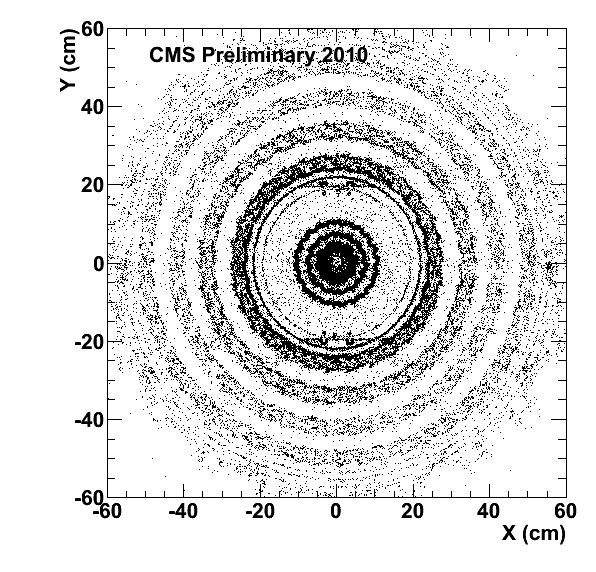
\includegraphics[width=0.40\textwidth]{fig/conversions/ptCut/data_xy.png}}
   \subfigure[]{
   \label{subfig:convXY_c}
    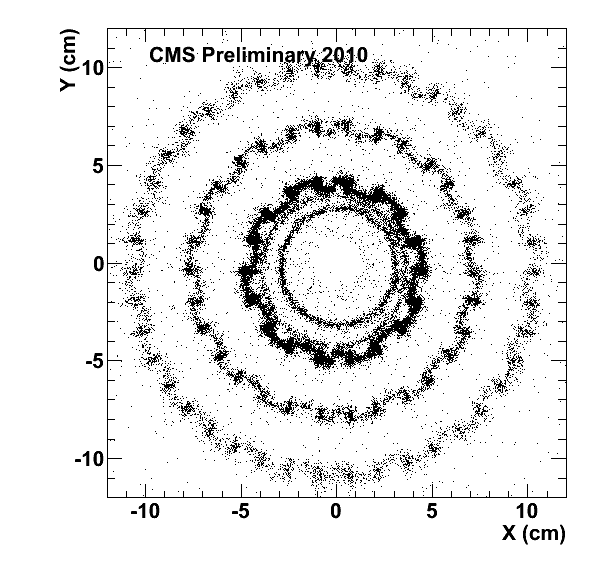
\includegraphics[width=0.40\textwidth]{fig/conversions/ptCut/data_xy_pixel_eta.png}}
    \caption{Conversion vertices reconstructed in CMS data in the $(x,y)$ plane for $|z|<26\cm$; zoom increases from (a) to (b). 
    Results were obtained on a sample corresponding to 1/nb of integrated luminosity where about 260 000 photon conversions were reconstructed. 
}
\label{fig:convXY}
\end{center}
\end{figure}
%
The  $(z, R)$  view of conversion vertices reconstructed in data is  shown in Fig.~\ref{fig:convRZ};  the less populated
areas  around $|\eta|\sim1.2$ corresponds to transition regions between the Tracker
barrel and endcap sub-components where the larger amount of passive material and the change in the active material topology makes more difficult the reconstruction of displaced vertexes. 
The dedicated seeding described in Sec.~\ref{sec:newSeedingStep} provides a reasonable increase of efficiency, as it will be shown later.


\begin{figure}[h!]
  \begin{center}
     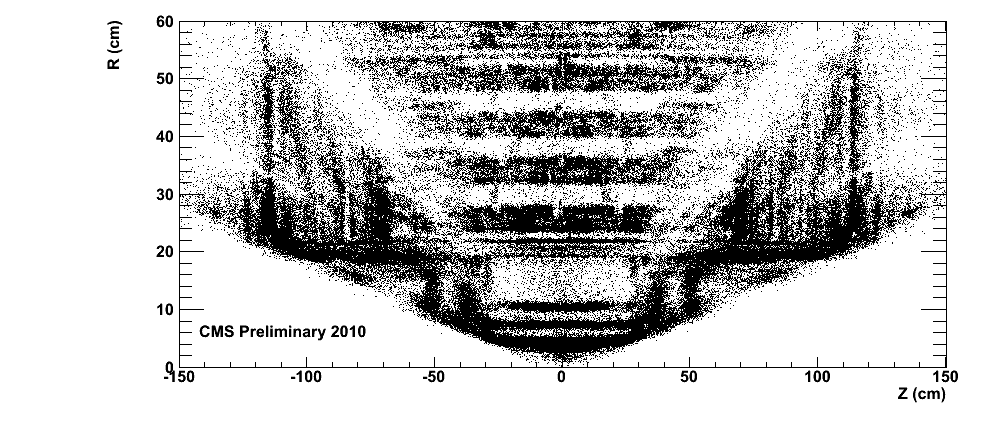
\includegraphics[width=17cm,height=5.7cm]{fig/conversions/ptCut/data_rz.png}
      \caption{Conversion vertices reconstructed in CMS data in the $(z,R)$ plane.}
    \label{fig:convRZ}
  \end{center}
\end{figure}


%\subsection{Radiative decay of heavy flavor particles}

Another field that takes advantage of the photon conversion reconstruction is the study of heavy quarkonia states. These bound states of charm and bottom quark-antiquark pairs play an important role in the detailed understanding of quantum-chromodynamics 
(QCD), the theory describing the strong interactions among elementary particles. 
A quantitative understanding of the mechanisms of quarkonium production can
be provided by measurements of the production cross sections and 
polarizations of P-wave quarkonia, such as the $\chi_{cJ}$ and the 
$\chi_{bJ}$ states, especially at the high transverse momentum ranges
reachable in high-energy proton colliders.
The CMS experiment is well capable 
of detecting and accurately reconstructing the $\chi_{c}$ ($\chi_{b}$)
states, through their radiative decays to the $\JPsi$ ($\Upsilon$)
state with the low-energy photons being detected through their conversion 
in electron-positron pairs~\cite{chic}. 

At  low energies (rarely above 
$2.5\GeV$ in the laboratory), the calorimetric
measurements do not have precisions comparable to those obtainable
when the photon energy is measured through the tracking of the 
electron-positron pair originating from a conversion of the photon.
Figure~\ref{fig:chic} shows the invariant mass distribution for $\chi_c$ candidates
observed through their radiative decay in $\JPsi + \cPgg$. The excellent momentum resolution of the reconstructed photon conversions translates in a mass resolution of less then 10~MeV, what is enough to disentangle  the states $\Chione$ and $\Chitwo$, whose masses differ by only 45\MeV.
%
Furthermore, the  converted photons have an accurate assignment of the interaction vertex where they come from, allowing  to limit the combinatorial background in the invariant mass spectrum of Fig.~\ref{fig:chic}
rejecting wrong combinations of  dimuons  plus  photons produced in different $pp$ collisions at the same bunch crossing (something especially important in the
presence of a large number of pileup collisions). 


The drawback of the usage of photon conversions for a physics measurement 
is the reduced yield caused by the low efficiency of their reconstruction as pairs of low momentum tracks displaced with respect to the beam axis. Typical efficiency is of the order of $0.1 \div 5\%$ for photon \pt  $< 5 \GeVc$. It is then evident that any new algorithm contributing to increase this efficiency has a direct impact in the physics analyses.





\begin{figure}[h]
  \begin{center}
    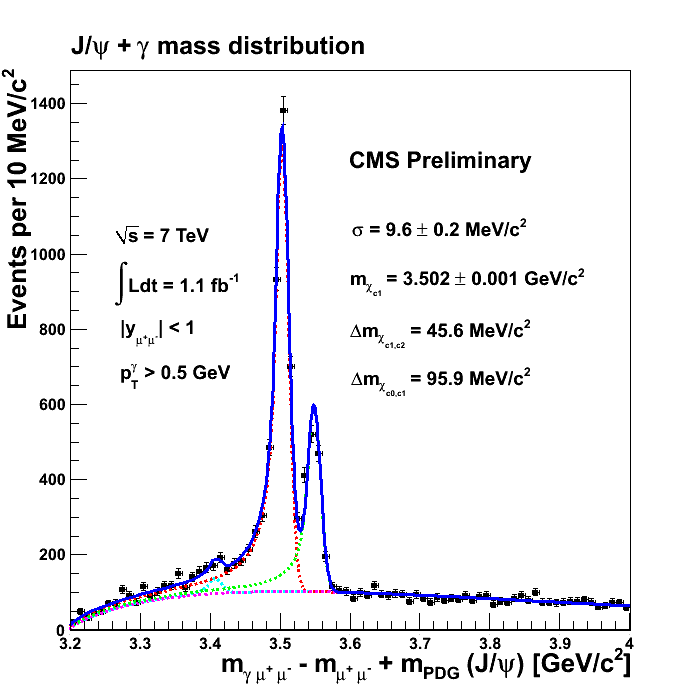
\includegraphics[width=0.6\textwidth]{fig/Chic1fb.png}
    \label{fig:chic}
   \caption{Invariant mass spectrum for $\chi_c$ candidates  reconstructed through their radiative decay to $\JPsi + \cPgg$.}
     \end{center}
\end{figure} 


%---------------------------------------------------------------------------------------------------------------

\section{Photon Conversion Reconstruction}
\label{standard}


Reconstruction of converted photons is therefore a crucial step in the physics program of CMS, and  algorithms have been developed, which exploit the conversion pair signature to distinguish genuine pairs from fake pairs.
%
Photon conversions are characterized by a pair of
oppositely charged secondary tracks, originating from the photon conversion vertex with an
invariant mass consistent with zero,  which are therefore parallel
to each other at production vertex. The electron-positron pair, then,
opens only in the transverse plane because of the solenoidal magnetic field.
The general reconstruction approach is to preselect pairs of oppositely charged tracks satisfying the quality and topological criteria of photon conversions and to fit each of these pairs by a 3D-constrained kinematic vertex 
fitter that imposes the two tracks to be parallel at the vertex. 

Two methods are used in CMS to generate the collection of potential conversion tracks: the ECAL-seeded conversion method~\cite{EGM-10-005}  and the combined conversion method. The former starts from calorimetric clusters and is optimized for very displaced conversion vertexes as well as high-\pt photons ($p_{\rm T} >10\GeVc$).
To reconstruct photon conversions within a soft-\pt spectrum (such as the majority of the photons from $\pi^0$ decays in minimum bias events or from quarkonia excited states) the ECAL cluster-driven track cannot be used,  because the electron pairs from conversions are very unlikely to reach the electromagnetic calorimeter.
Therefore  conversions need to be reconstructed pairing tracks from the  CMS general track and electron track (GSF) collections.
The general track collection is 
 an inclusive collection of   tracks resulting from an iterative procedure~\cite{TRK-10-001} to incorporate increasingly displaced and/or low-\pt tracks.
%
 The GSF (Gaussian Sum Filter) track collection is specific for electron candidates. It employs a 
  weighted  	sum of Gaussian components to model the non-Gaussian energy loss distribution for electrons passing through the material. 
%
The collection of tracks in the combined conversion method is obtained from a combination of general tracks,  conversion ECAL-seeded tracks and GSF tracks.

%---------------------------------------------------------------------------------------------------------------

\section{Tracking algorithm for photon conversions}
\label{sec:newSeedingStep}
 

The standard CMS tracking is made of consecutive iterative steps designed to obtain high efficiency and low fake rate for
tracks coming either from the primary vertex or from displaced decay
vertices while maintaining the overall computing time within the
requirements of the CMS offline reconstruction.
Because of this constraint, the standard implementation is not optimal
to reconstruct with high efficiency tracks from photon conversions
since the cuts applied in the standard
reconstruction are too tight for these processes. Those
tracks have usually very low momentum and, especially for displaced
vertices at large radii, they have a large transverse impact parameter.

Beside the soft-\pt spectrum of the majority of the photons produced at LHC, another reason why the conversion tracks have low momentum is the asymmetric distribution of the energy among the $e^+e^-$ pairs~\cite{pdg}, implying that one lepton carries most of the photon energy, leaving the second lepton with a too low momentum to be reconstructed. As a result these photons are not found by the conversion finding algorithms because only one of the two tracks is missing, whereas the leading track has been reconstructed.

Exploiting this feature, we have developed a dedicated track reconstruction that recovers those photon conversions for which the 
leading  track has been already reconstructed. The leading track is used to drive the reconstruction of the second track, for this reason we refer to the algorithm as track-driven and to the leading track as the seeding track.

Our tracking algorithm is configured as an additional step of the CMS iterative tracking. Having to use all the available reconstructed tracks, it is the last to run after all the other standard iterative tracking steps.
%
Similarly to  the other steps, the track-driven algorithm starts from identifying trajectory seeds from which to build the full trajectories using the standard CMS tracking sequence, based on Kalman filter method in the pattern recognition and track refitting.
Trajectory seeds are built from pairs of hits
in the Pixel and/or in the Strip Tracker detectors. 
In order to reduce the number of hits to combine as well as to avoid to reconstruct already built tracks,  only hits not associated to other tracks are used in the seeding search.

Due to the massless photon, the tracks of the resulting electrons from a photon conversion are parallel to each other at the conversion vertex, and open in two opposite arcs of circumference in the  plane transverse to the CMS magnetic field ($(x,y)$ plane in Fig.~\ref{fig:algo}~\subref{subfig:algoXY}),
whereas they  remain parallel in the  longitudinal plane ($(z,r)$ plane in Fig.~\ref{fig:algo}~\subref{subfig:algoRZ}). This is a unique feature that is the basis of the algorithm we developed. 


\begin{figure}[]
\centering
\subfigure[]{
\label{subfig:algoXY}
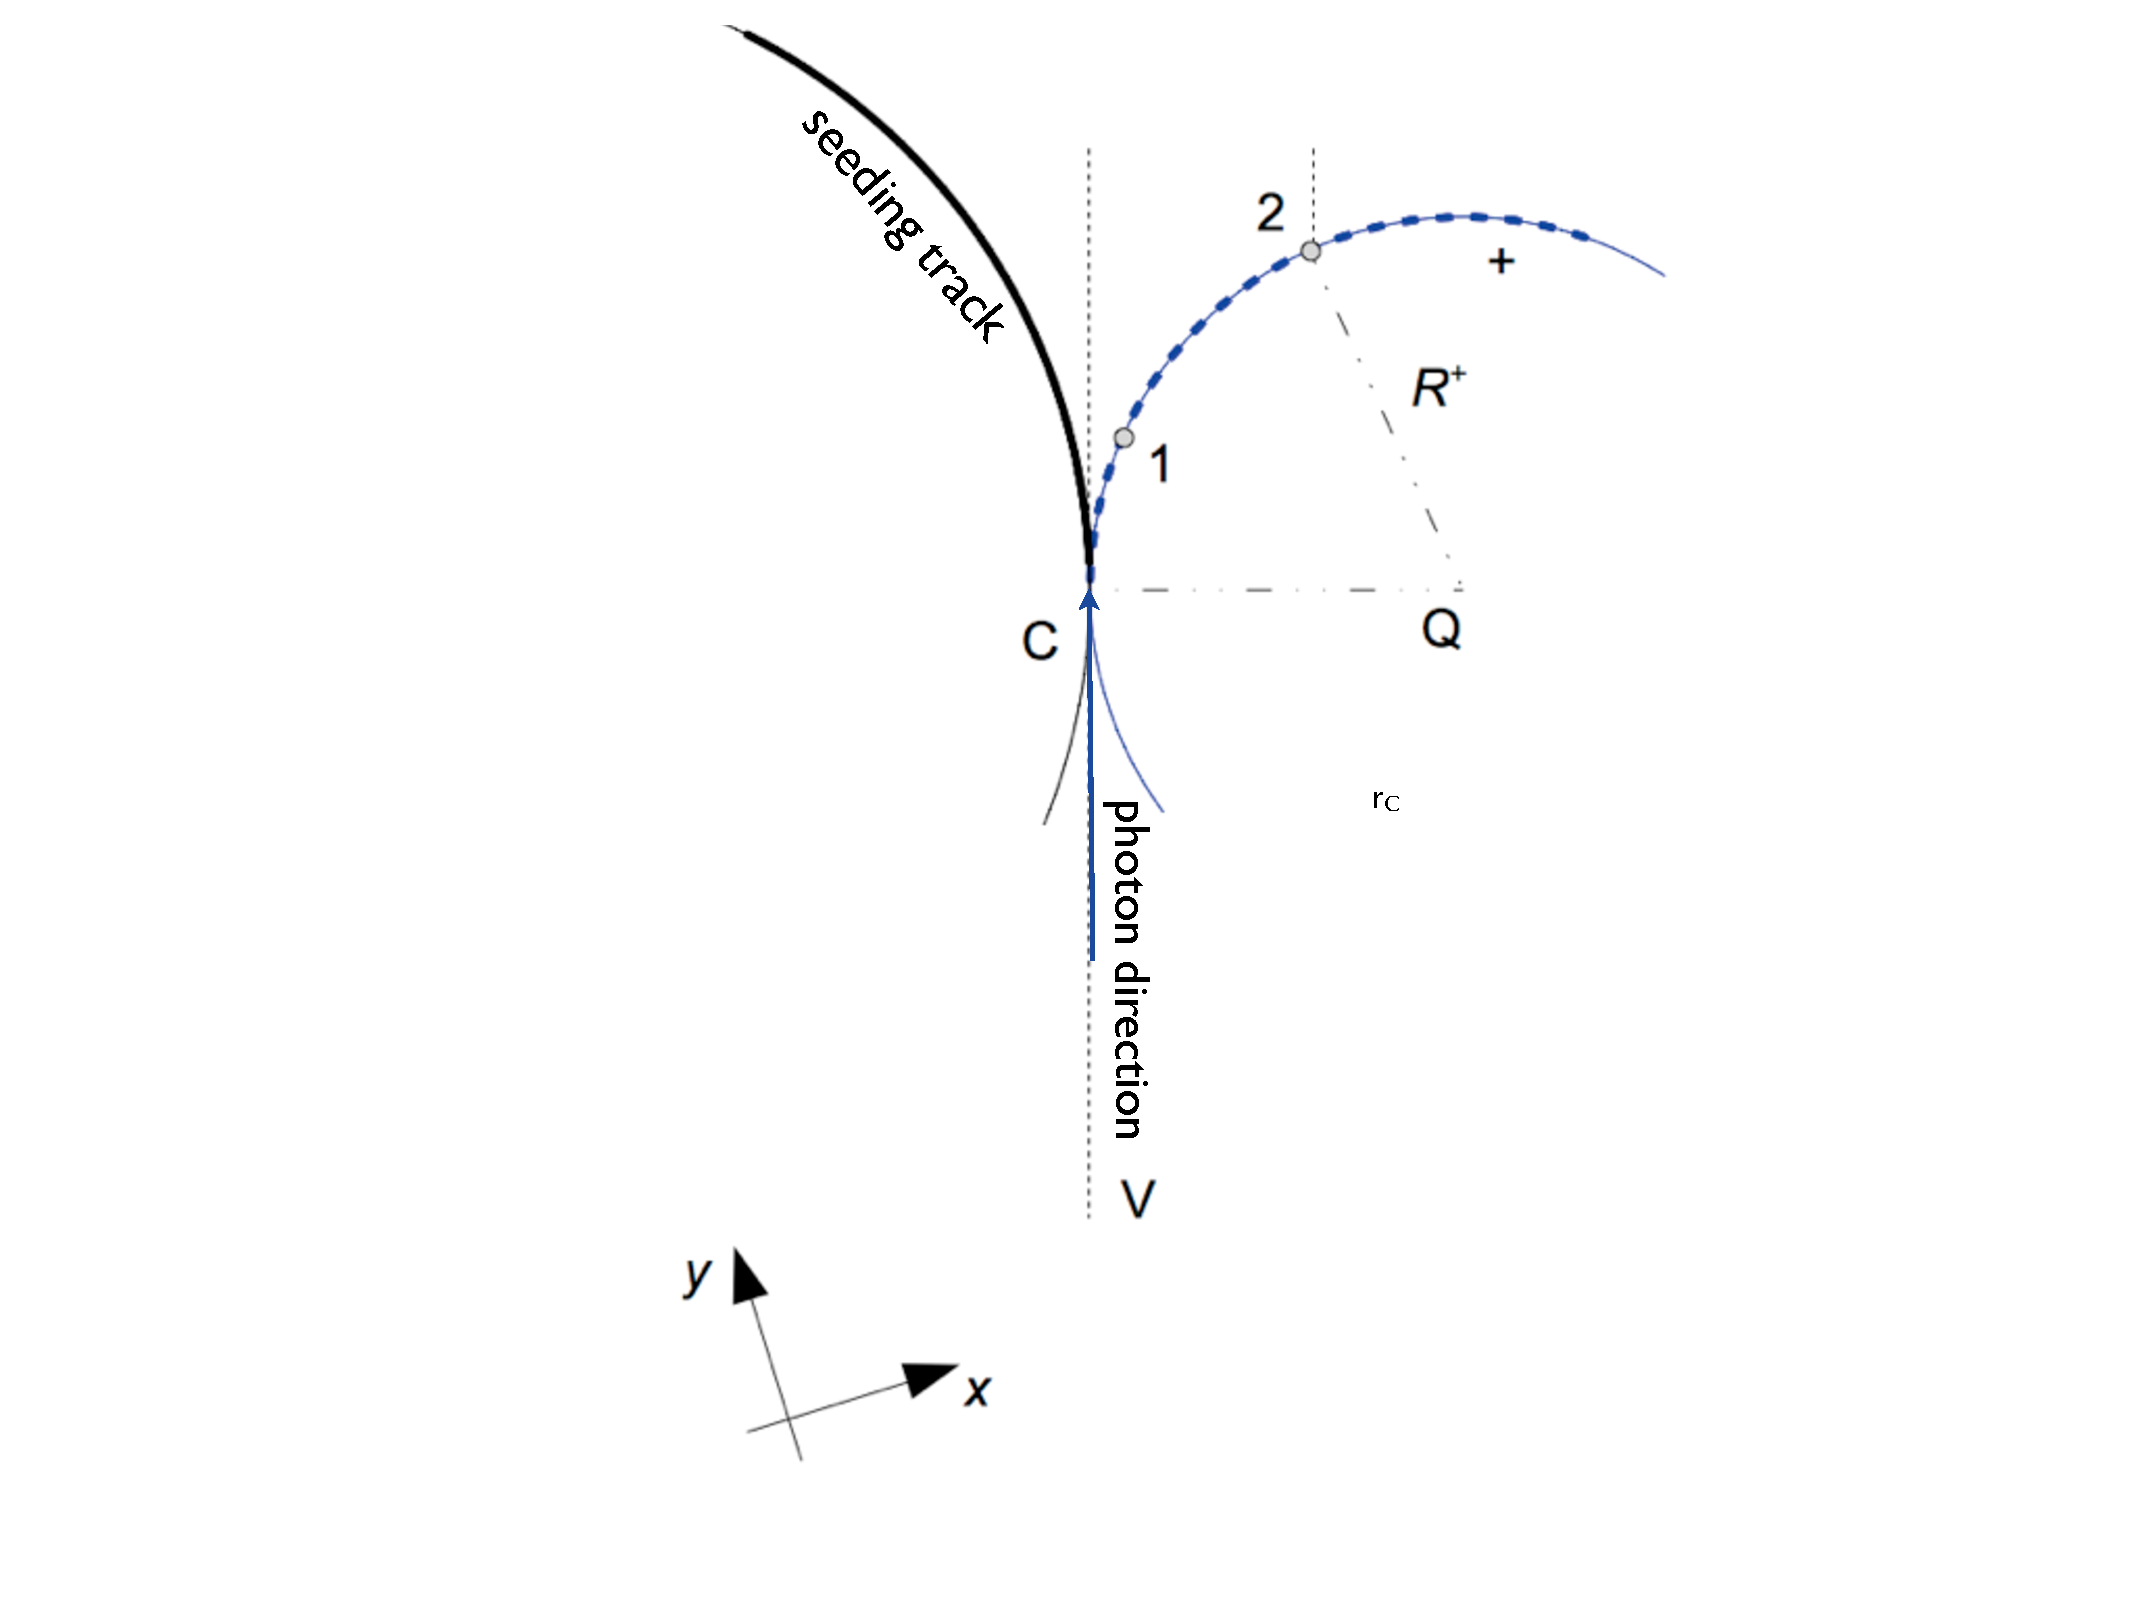
\includegraphics[trim=7cm 0cm 7cm 0cm, clip=true,width=.4\textwidth]{fig/singleLegAlgoXY.pdf}}
\subfigure[]{
\label{subfig:algoRZ}
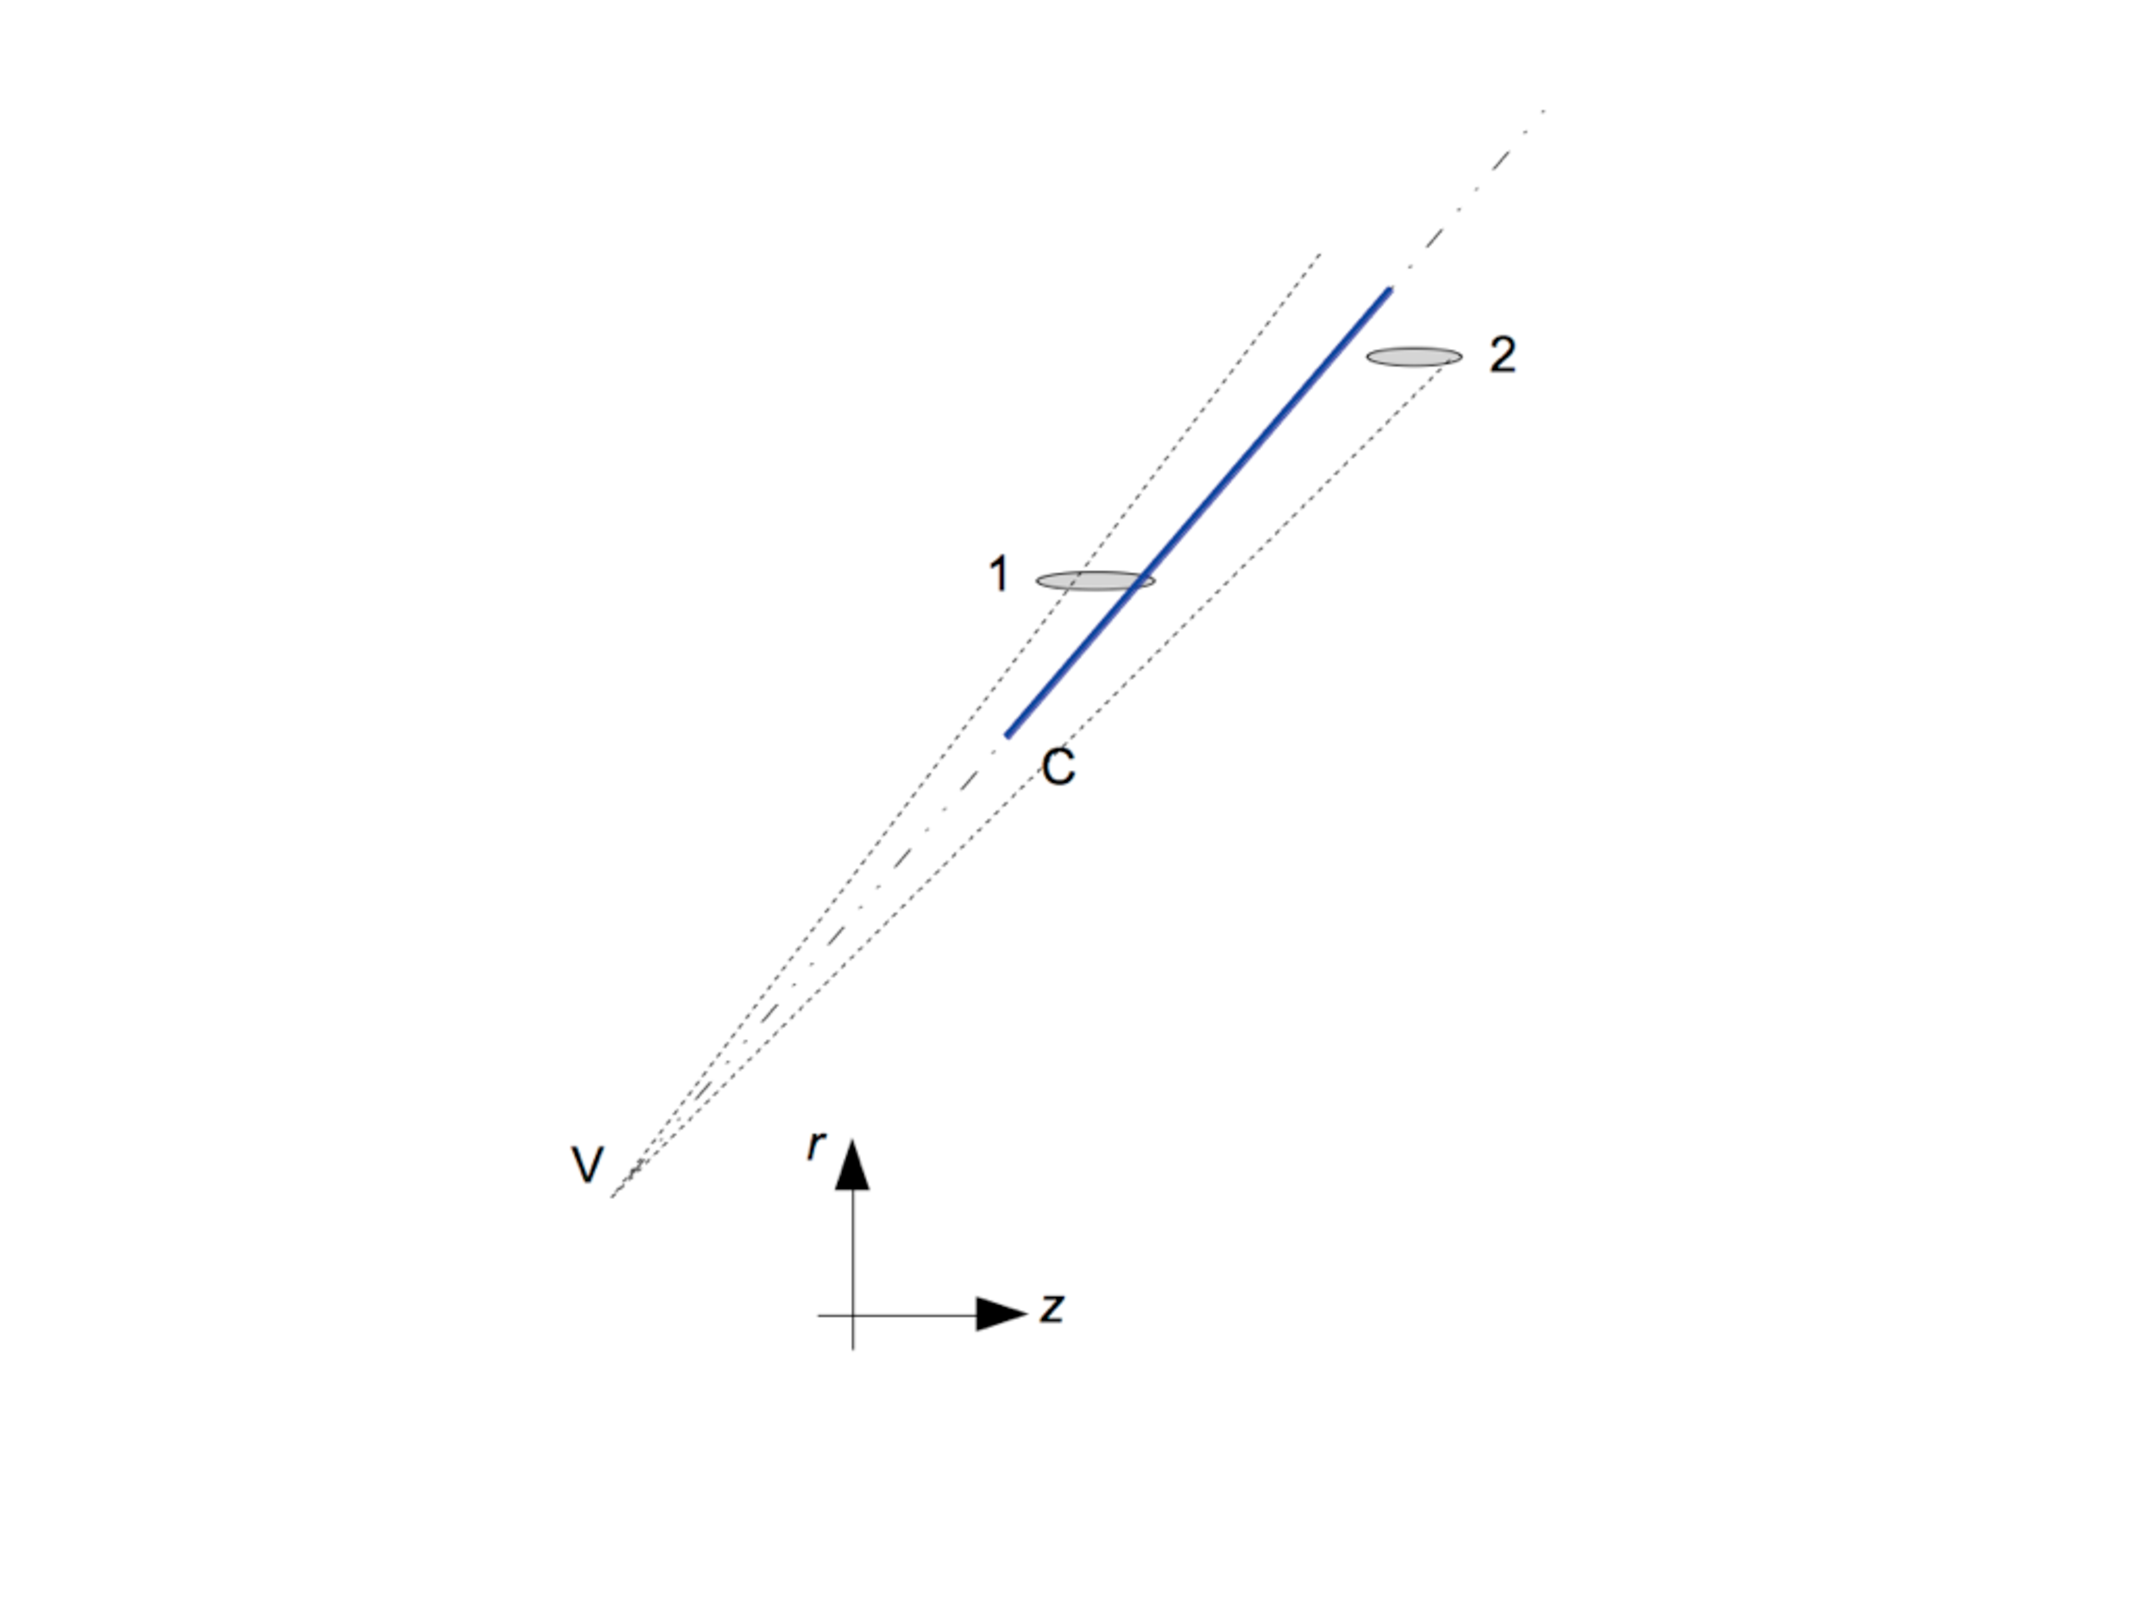
\includegraphics[trim=7cm 0cm 7cm 0cm, clip=true,width=.4\textwidth]{fig/singleLegAlgoRZ.pdf}}
\caption{Cartoon showing the photon conversion topology in a solenoidal magnetic field,
shown in the plane transverse  to the CMS magnetic field~\subref{subfig:algoXY}, as well as  in the longitudinal plane~\subref{subfig:algoRZ}.}

\label{fig:algo}
\end{figure}

Not all the tracks from  the standard collection are used to drive our seeding. The seeding tracks are selected applying the geometrical conditions imposed by the hypothesis of belonging to a prompt-photon conversion. 
%
As described in Fig.~\ref{fig:algo}~\subref{subfig:algoXY}, in the transverse plane the photon direction (VC) is tangent to both tracks in the conversion point C. Starting from a track and its associated primary vertex (V), with pure geometrical considerations the estimated position of the conversion vertex (C) is obtained. Given that a photon conversion happens in the material inside the tracker volume, from the beampipe onwards, tracks compatible with the conversion hypothesis cannot have the estimated vertex position (C) at a radial distance from the beamline ($\rm r_C$) inferior to the radius of the beampipe ($\rm r=3~cm$). Applying this condition, relaxed of 0.5~cm to take into account the resolution of our geometrical estimation,  prompt tracks from primary vertices are rejected, and only potential candidates from conversions are kept.

With the same approach, for a given seeding track  having  the estimated position of the conversion vertex at  $\rm r_C$ only the pairs of consecutive layers located at a radial distance from the beamline above $\rm r_C$ are used to build the hit pair seeds. 
%
Having to reconstruct a track of opposite charge respect to the seeding track, only hit pairs in the semi-plane defined by the VC direction and opposite to the seeding track are considered. The search is limited to an maximum opening angle -- with respect to the direction VC -- correlated to the minimum \pt to be reconstructed, that in our case is $100~\MeVc$.

The requirement that the two conversion tracks are parallel to the photon direction in the rz plane (Fig.~\ref{fig:algo}~\subref{subfig:algoRZ}) allows to further   reduce the number of hit combinations to keep into account, limiting the region of interest to a cone around the seeding track, such that the track extrapolated position to the hit surface is compatible with the hit position in 3 standard deviations.  


For each seeding track a collection of hit pairs satisfying the above requirements  is identified and used to construct the trajectory seeds, i.e. the proto-tracks providing the initial kinematic parameters needed for the trajectory propagation.
At least three points are requested to evaluate the 5 parameters of the initial kinematic, but only two hits are provided per hit pair, and some of them have a coarse resolution in the $z$ coordinate. The third measurement is provided, again, by the   estimated position of the conversion vertex (C). The coordinates of these three points in the $(x,y)$ plane allow to estimate the \pt of the trajectory seed. The direction of the trajectory seed in the $(z,R)$ plane is imposed parallel to the seeding track.

Seeds are then
propagated outward, adding compatible hits and updating the trajectory
until either the detector boundary is reached, or no additional
compatible hits can be found.  In the final stage, the collection of
hits is fit to obtain the best estimate of the track parameters.

\section{Results}

The impact of the dedicated tracking algorithm  to the reconstruction of photon conversions
 can be seen on Fig.~\ref{fig:effPerf} 
showing the contribution of the different tracking steps to the photon conversion
reconstruction as estimated by the simulation  for a detector region  $|\eta|<1.4$.
The additional step increases by more than a factor two the number of conversions at large radii -- outside the Pixel detector region -- and contributes significantly ($\sim 20\%$) in the Pixel detector layers. 
 At the same time the additional number of reconstructed fake photon conversions is kept low (Fig.~\ref{fig:effPerf}~\subref{subfig:fakeBarrel}), thanks to the demanding geometrical requirements adopted.
 

 Table ~\ref{tab:perfTable} summarises the reconstruction performance of our algorithm in terms of the increased number of true and fake photon conversions, distinguishing among barrel and endcap regions as well as among conversions undergone in the Pixel detector ($r < 15 \rm cm$) or in the remaining Tracker volume.
 
 %
  

\begin{figure}[h]
\centering
\subfigure[]{
\label{subfig:effBarrel}
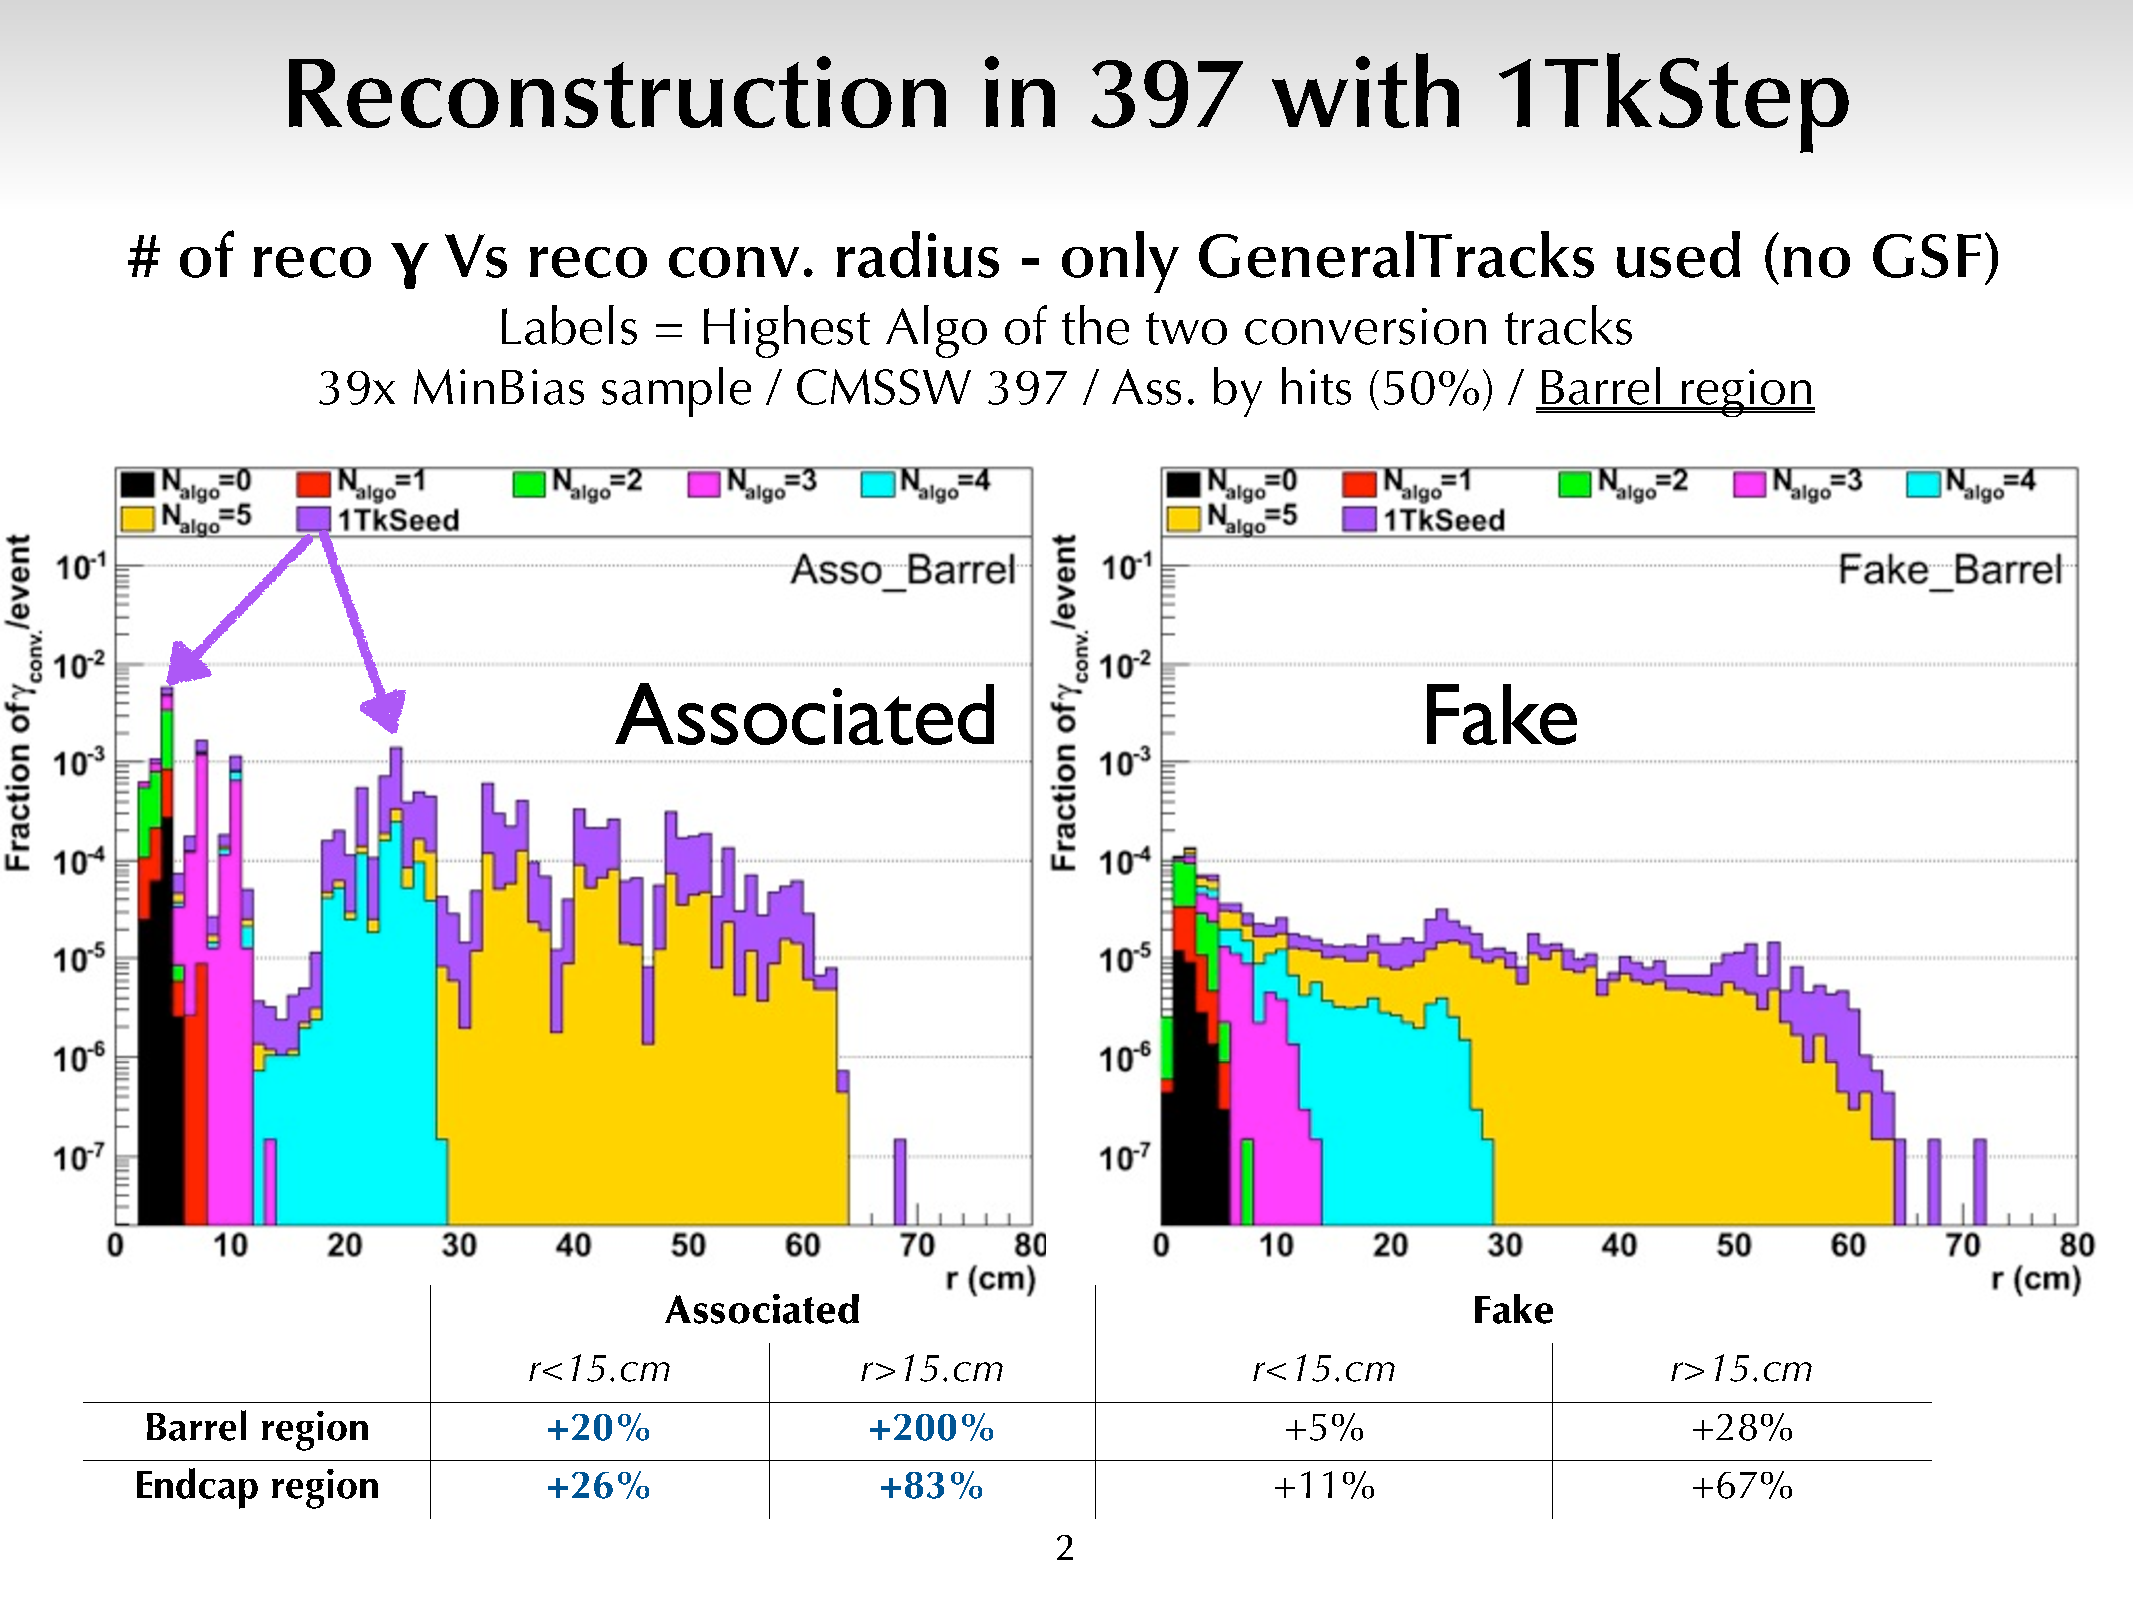
\includegraphics[trim=0cm 5.2cm 18.5cm 7.5cm, clip=true,width=.4\textwidth]{fig/singleLegBarrelEffect.pdf}}
\subfigure[]{
\label{subfig:fakeBarrel}
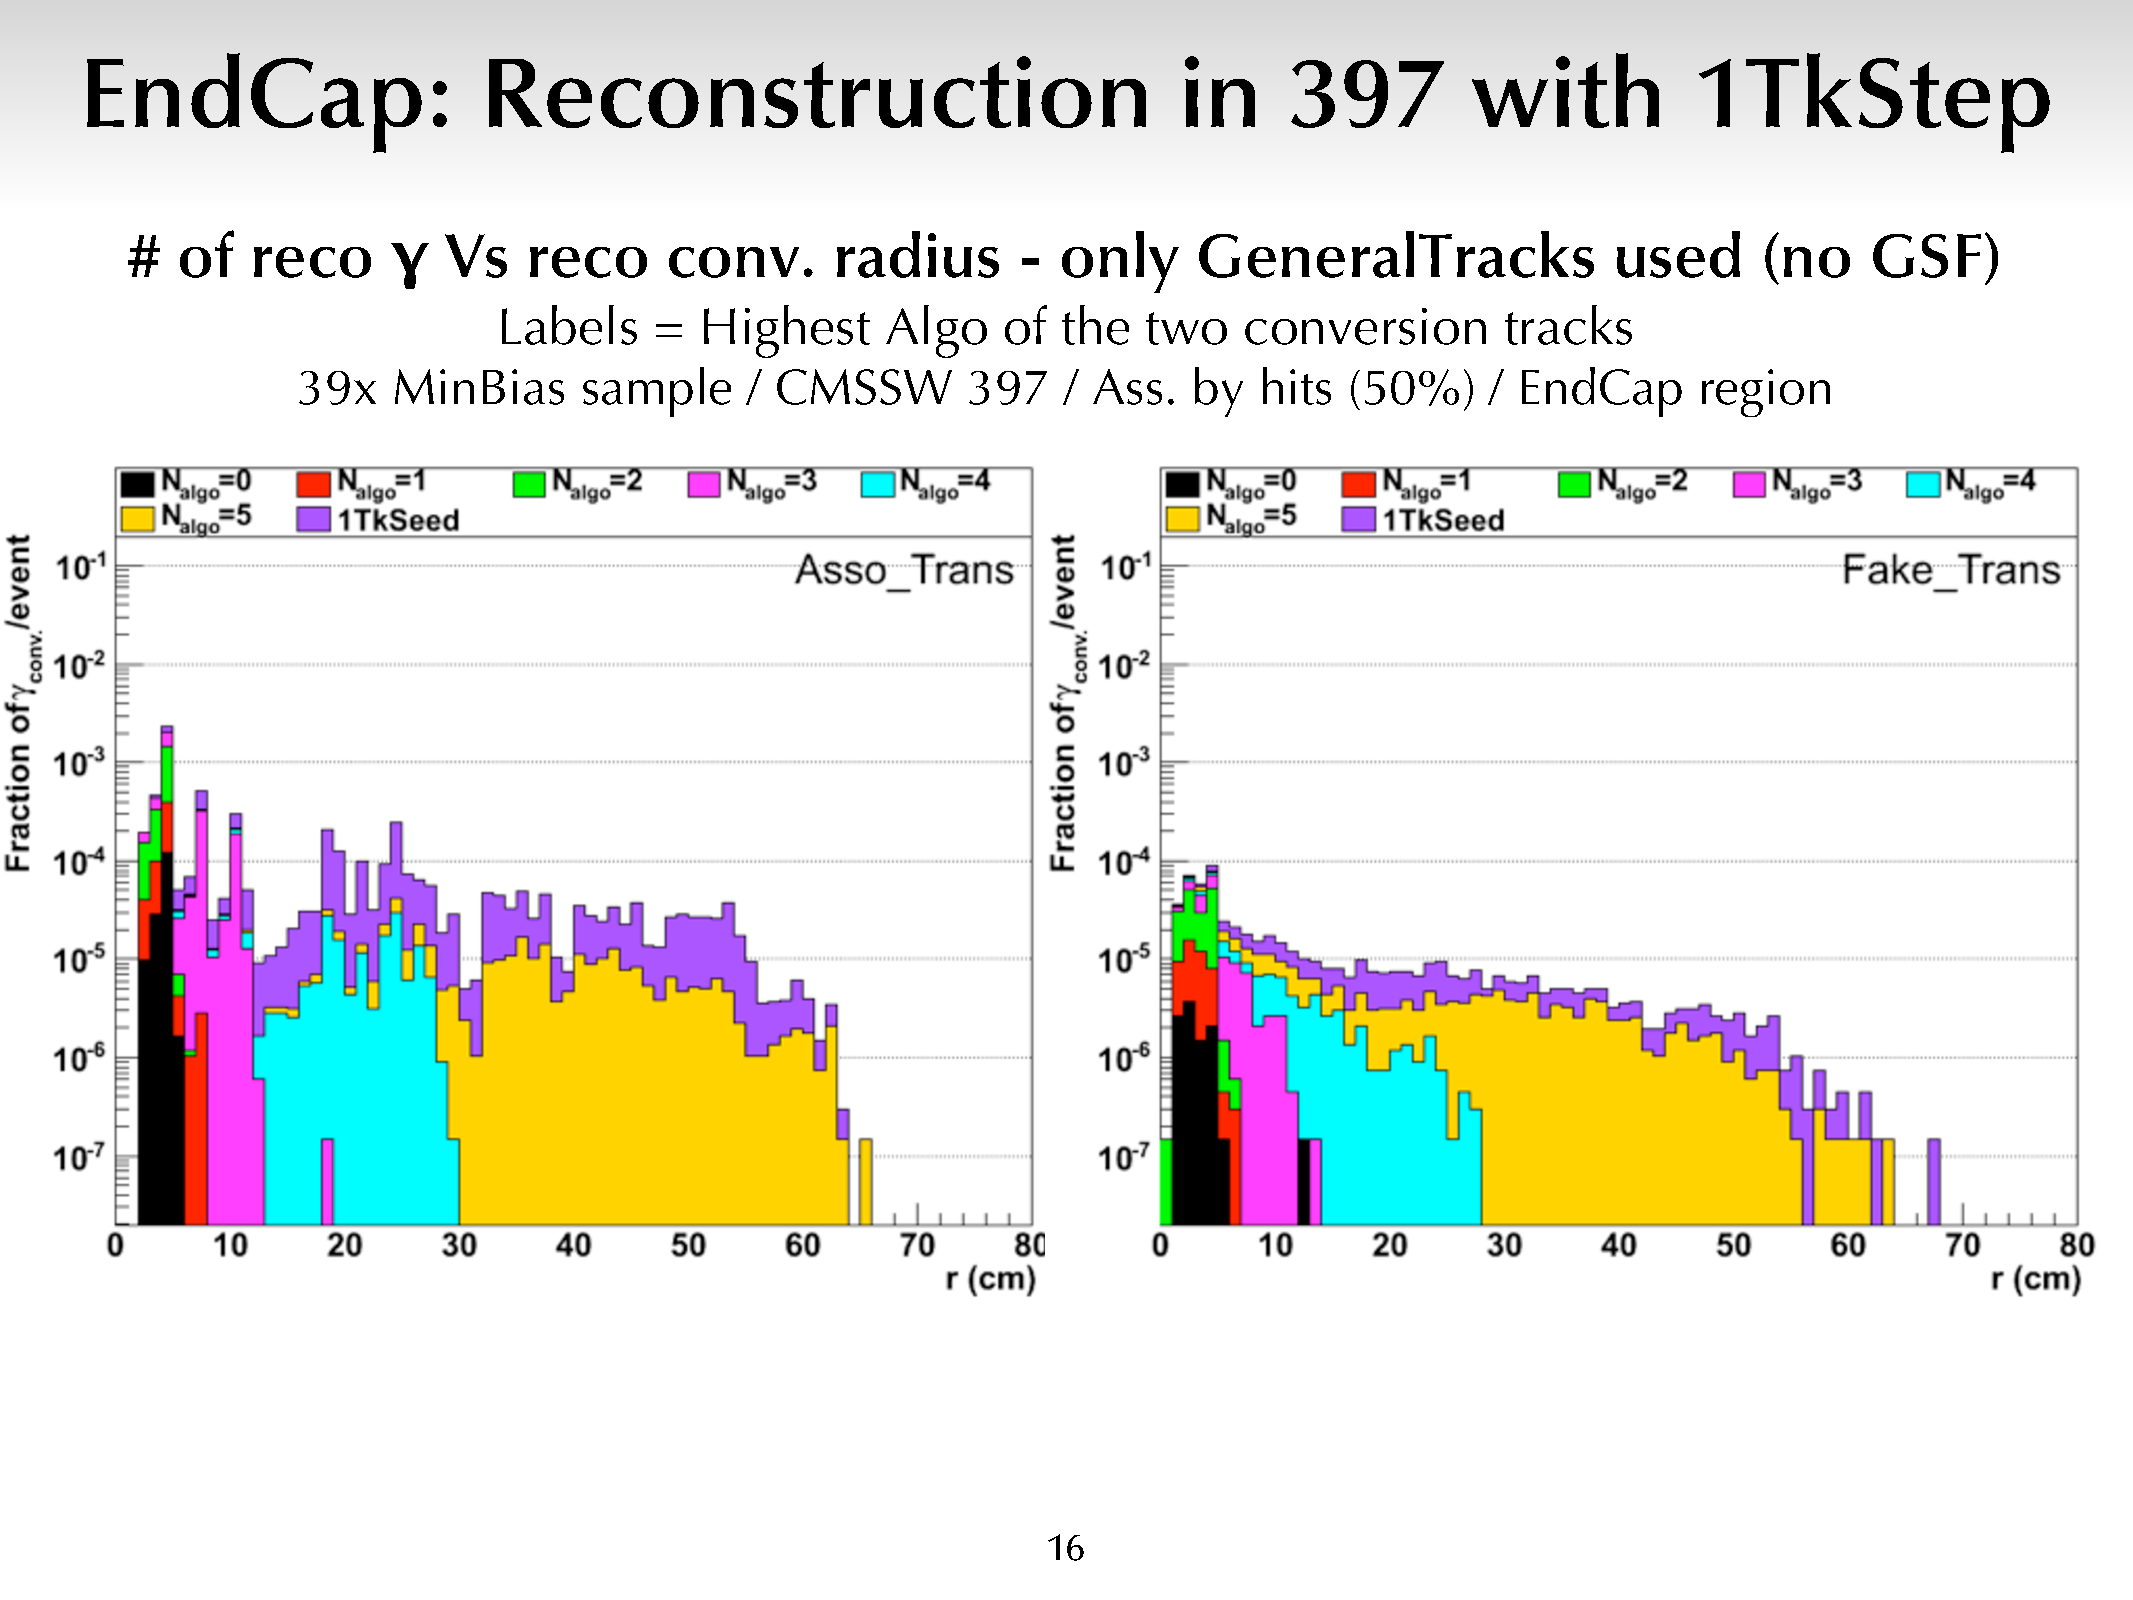
\includegraphics[trim=18.5cm 5.2cm 0cm 7.5cm, clip=true,width=.4\textwidth]{fig/singleLegEndCapEffect.pdf}}
\caption{Fraction of the reconstructed photon conversions per event as  a function of the radial position of the conversion vertex,   for  $|\eta|<1.4$ , as estimated
from simulation. The different colors correspond to the standard reconstruction algorithms only (green) and to the contribution of the new reconstruction algorithm (purple).}
\label{fig:effPerf}
\end{figure}


%\begin{figure}[h]
%\centering
%\subfigure[]{
%\label{subfig:fakeBarrel}
%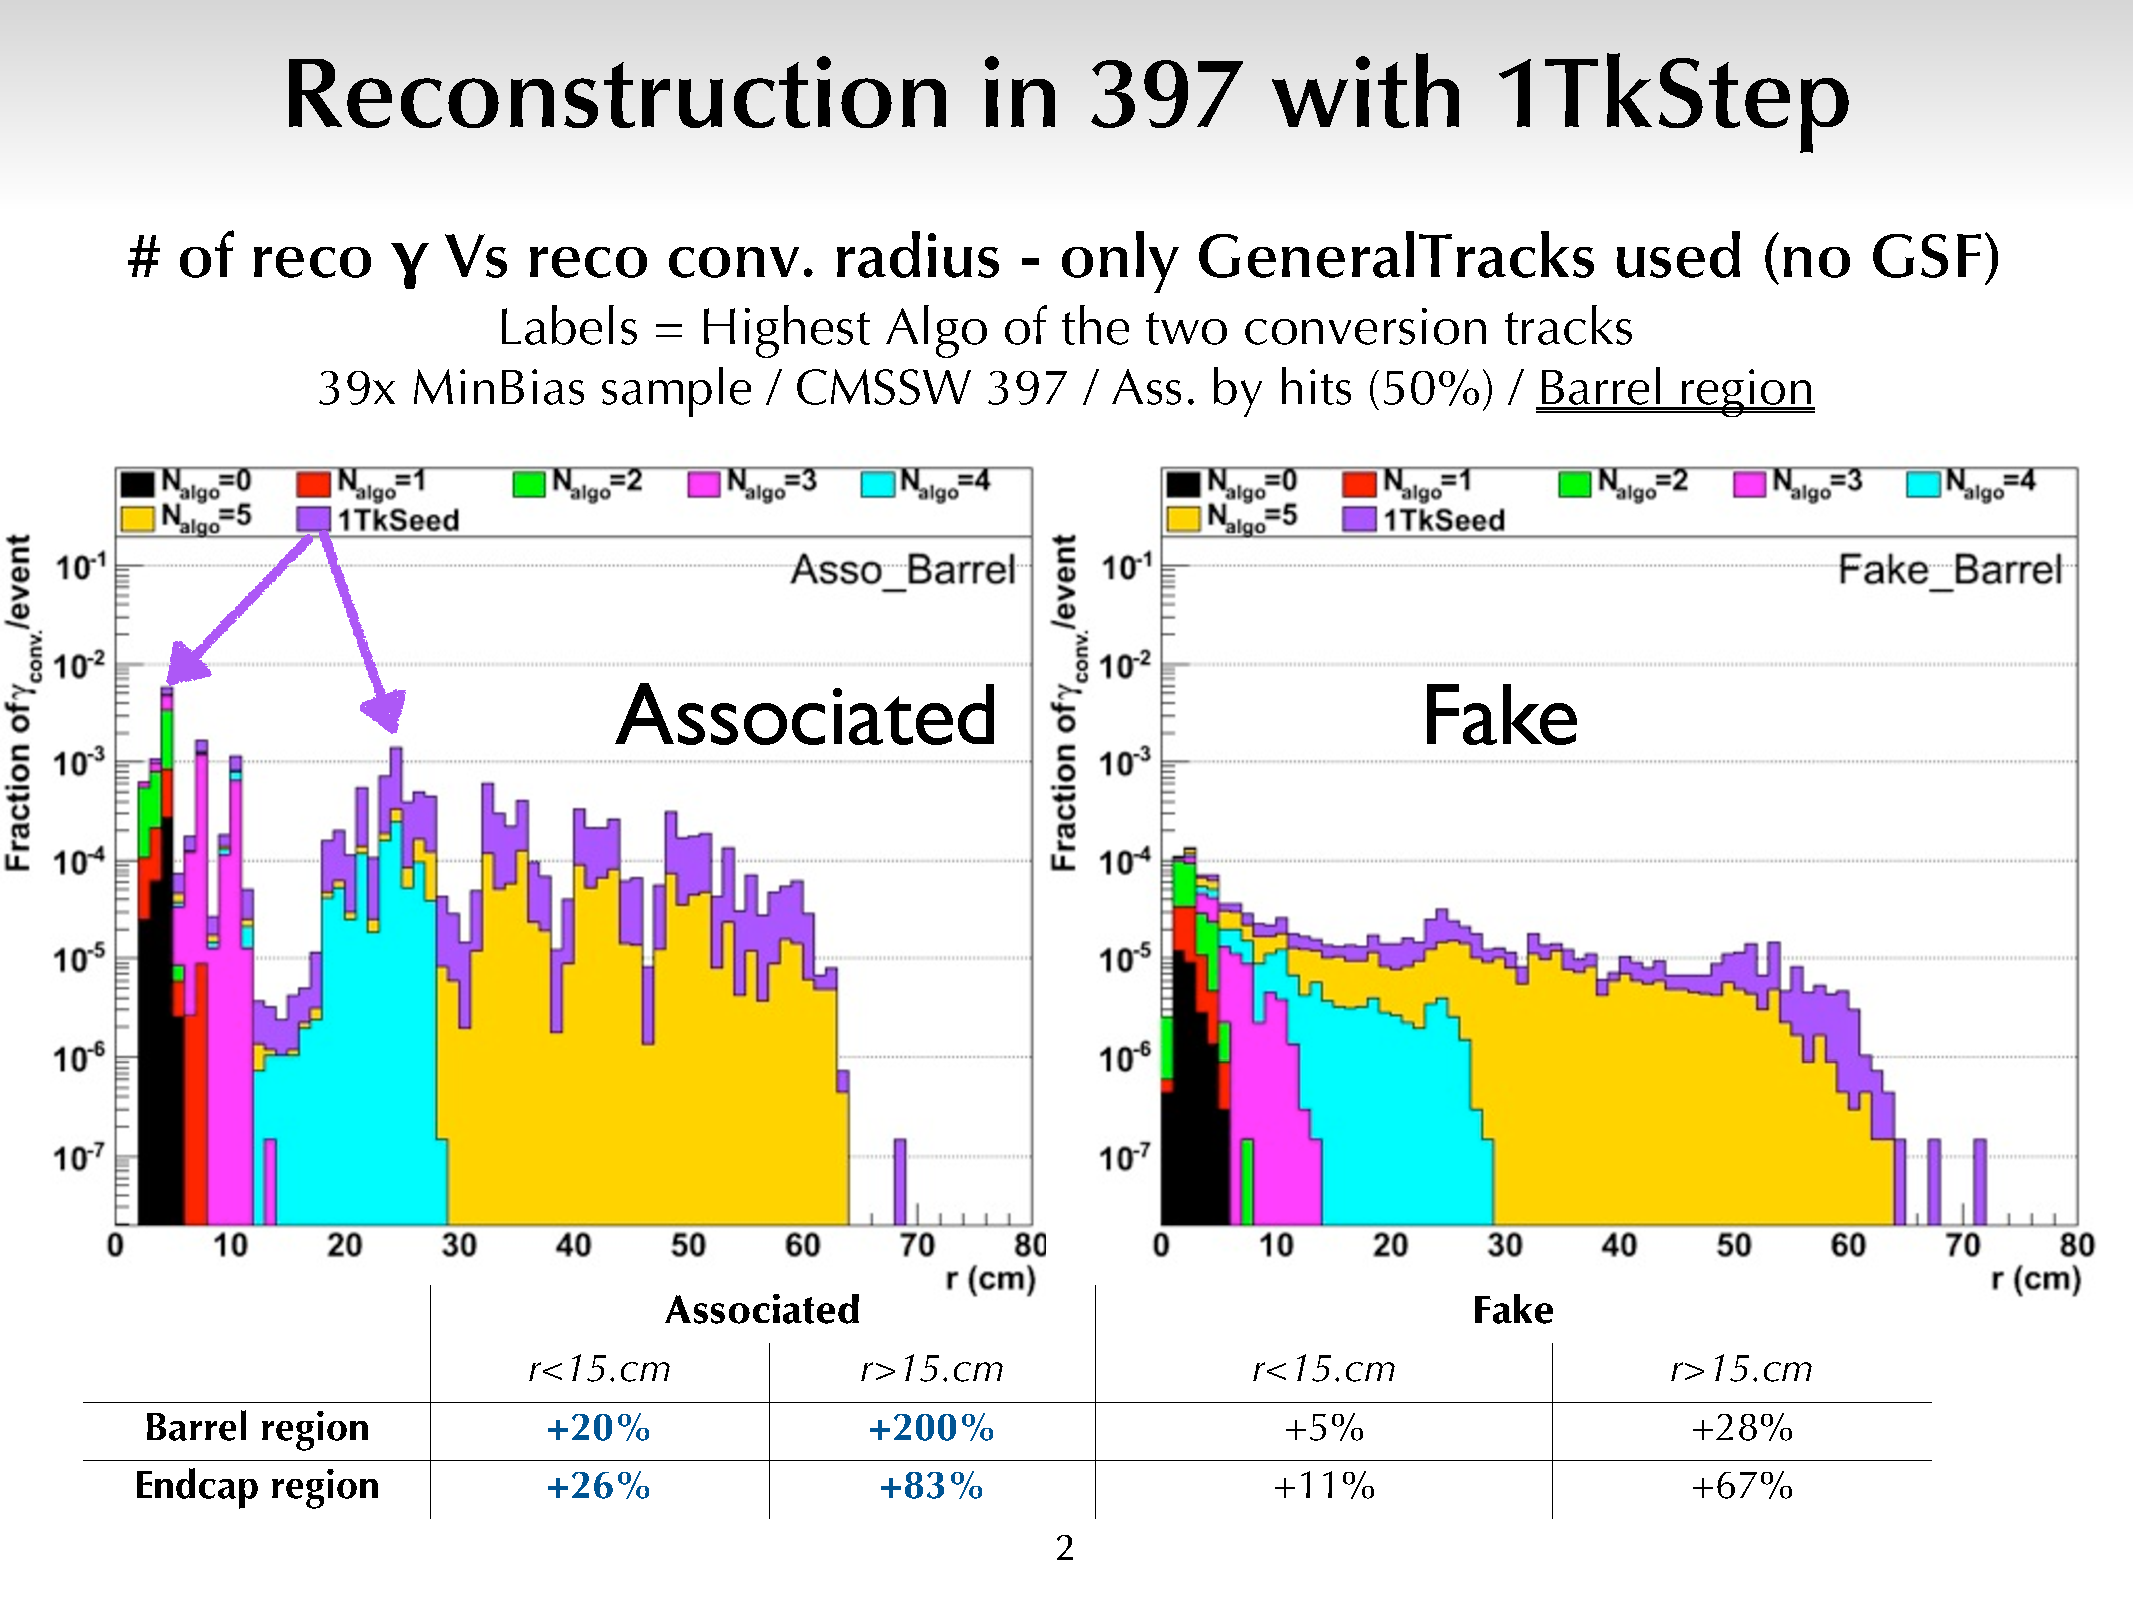
\includegraphics[trim=18.5cm 5.2cm 0cm 7.5cm, clip=true,width=.4\textwidth]{fig/singleLegBarrelEffect.pdf}}
%\subfigure[]{
%\label{subfig:fakeEndCap}
%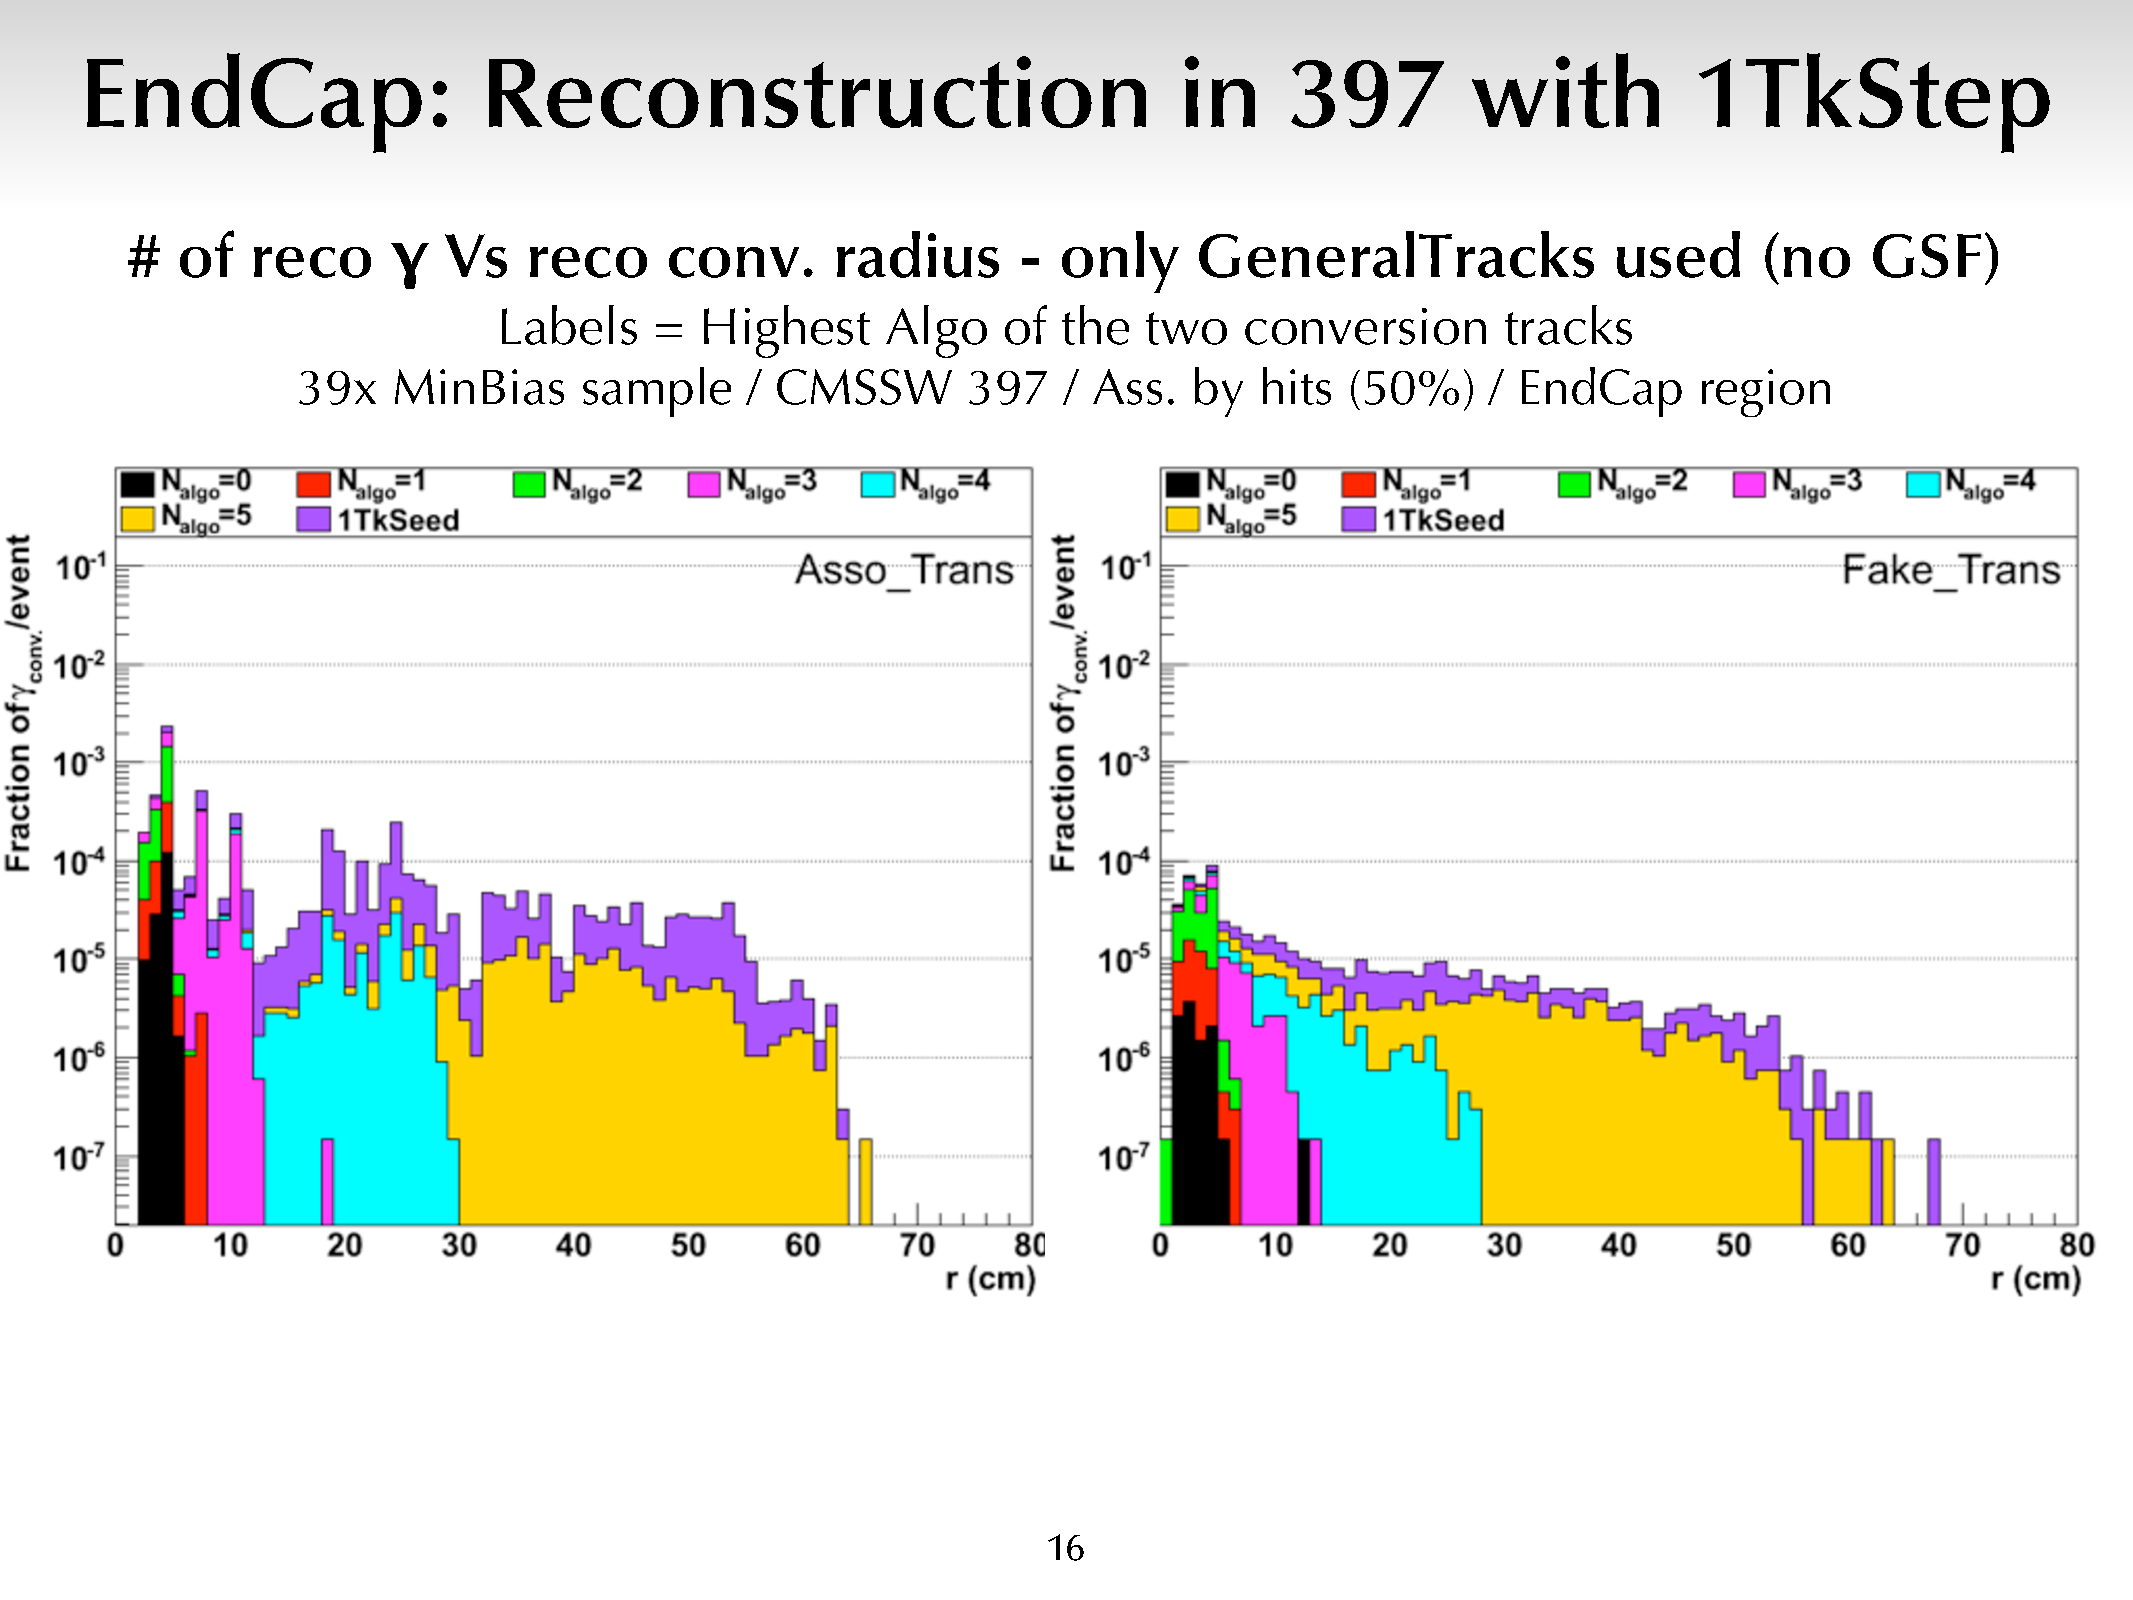
\includegraphics[trim=18.5cm 5.2cm 0cm 7.5cm, clip=true,width=.4\textwidth]{fig/singleLegEndCapEffect.pdf}}
%\caption{Fraction of the reconstructed fake photon conversions per event as  a function of the radial position of the conversion vertex, for the barrel~\subref{subfig:fakeBarrel} and the endcap~\subref{subfig:fakeEndCap} regions, as estimated
%from simulation. The different colors correspond to the largest
%iterative step needed to reconstruct the tracks at the vertex.}
%\label{fig:fakePerf}
%\end{figure}


\begin{table}[htdp]
\caption{Reconstruction performance of the dedicated algorithm in terms of the increase fraction of true and fake photon conversions, distinguishing among barrel and endcap regions as well as among conversions undergone in the Pixel detector ($r < 15 \rm cm$) or in the remaining Tracker volume.
}
\begin{center}
\begin{tabular}{c|c|c|c|c}
& \multicolumn{2}{c}{true} & \multicolumn{2}{|c}{false}  \\
& $r < 15 \rm cm$ & $r \ge 15 \rm cm$ & $r < 15 \rm cm$ & $r \ge 15 \rm cm$ \\
\hline
barrel & +20\% & +200\% & +5\% & +28\% \\
\hline
endcap & +26\% & +83\% & +11\% & +67\% 
\end{tabular}
\end{center}
\label{tab:perfTable}
\end{table}%

\begin{figure}[h]
\centering
\subfigure[]{
\label{subfig:RZCoverageStd}
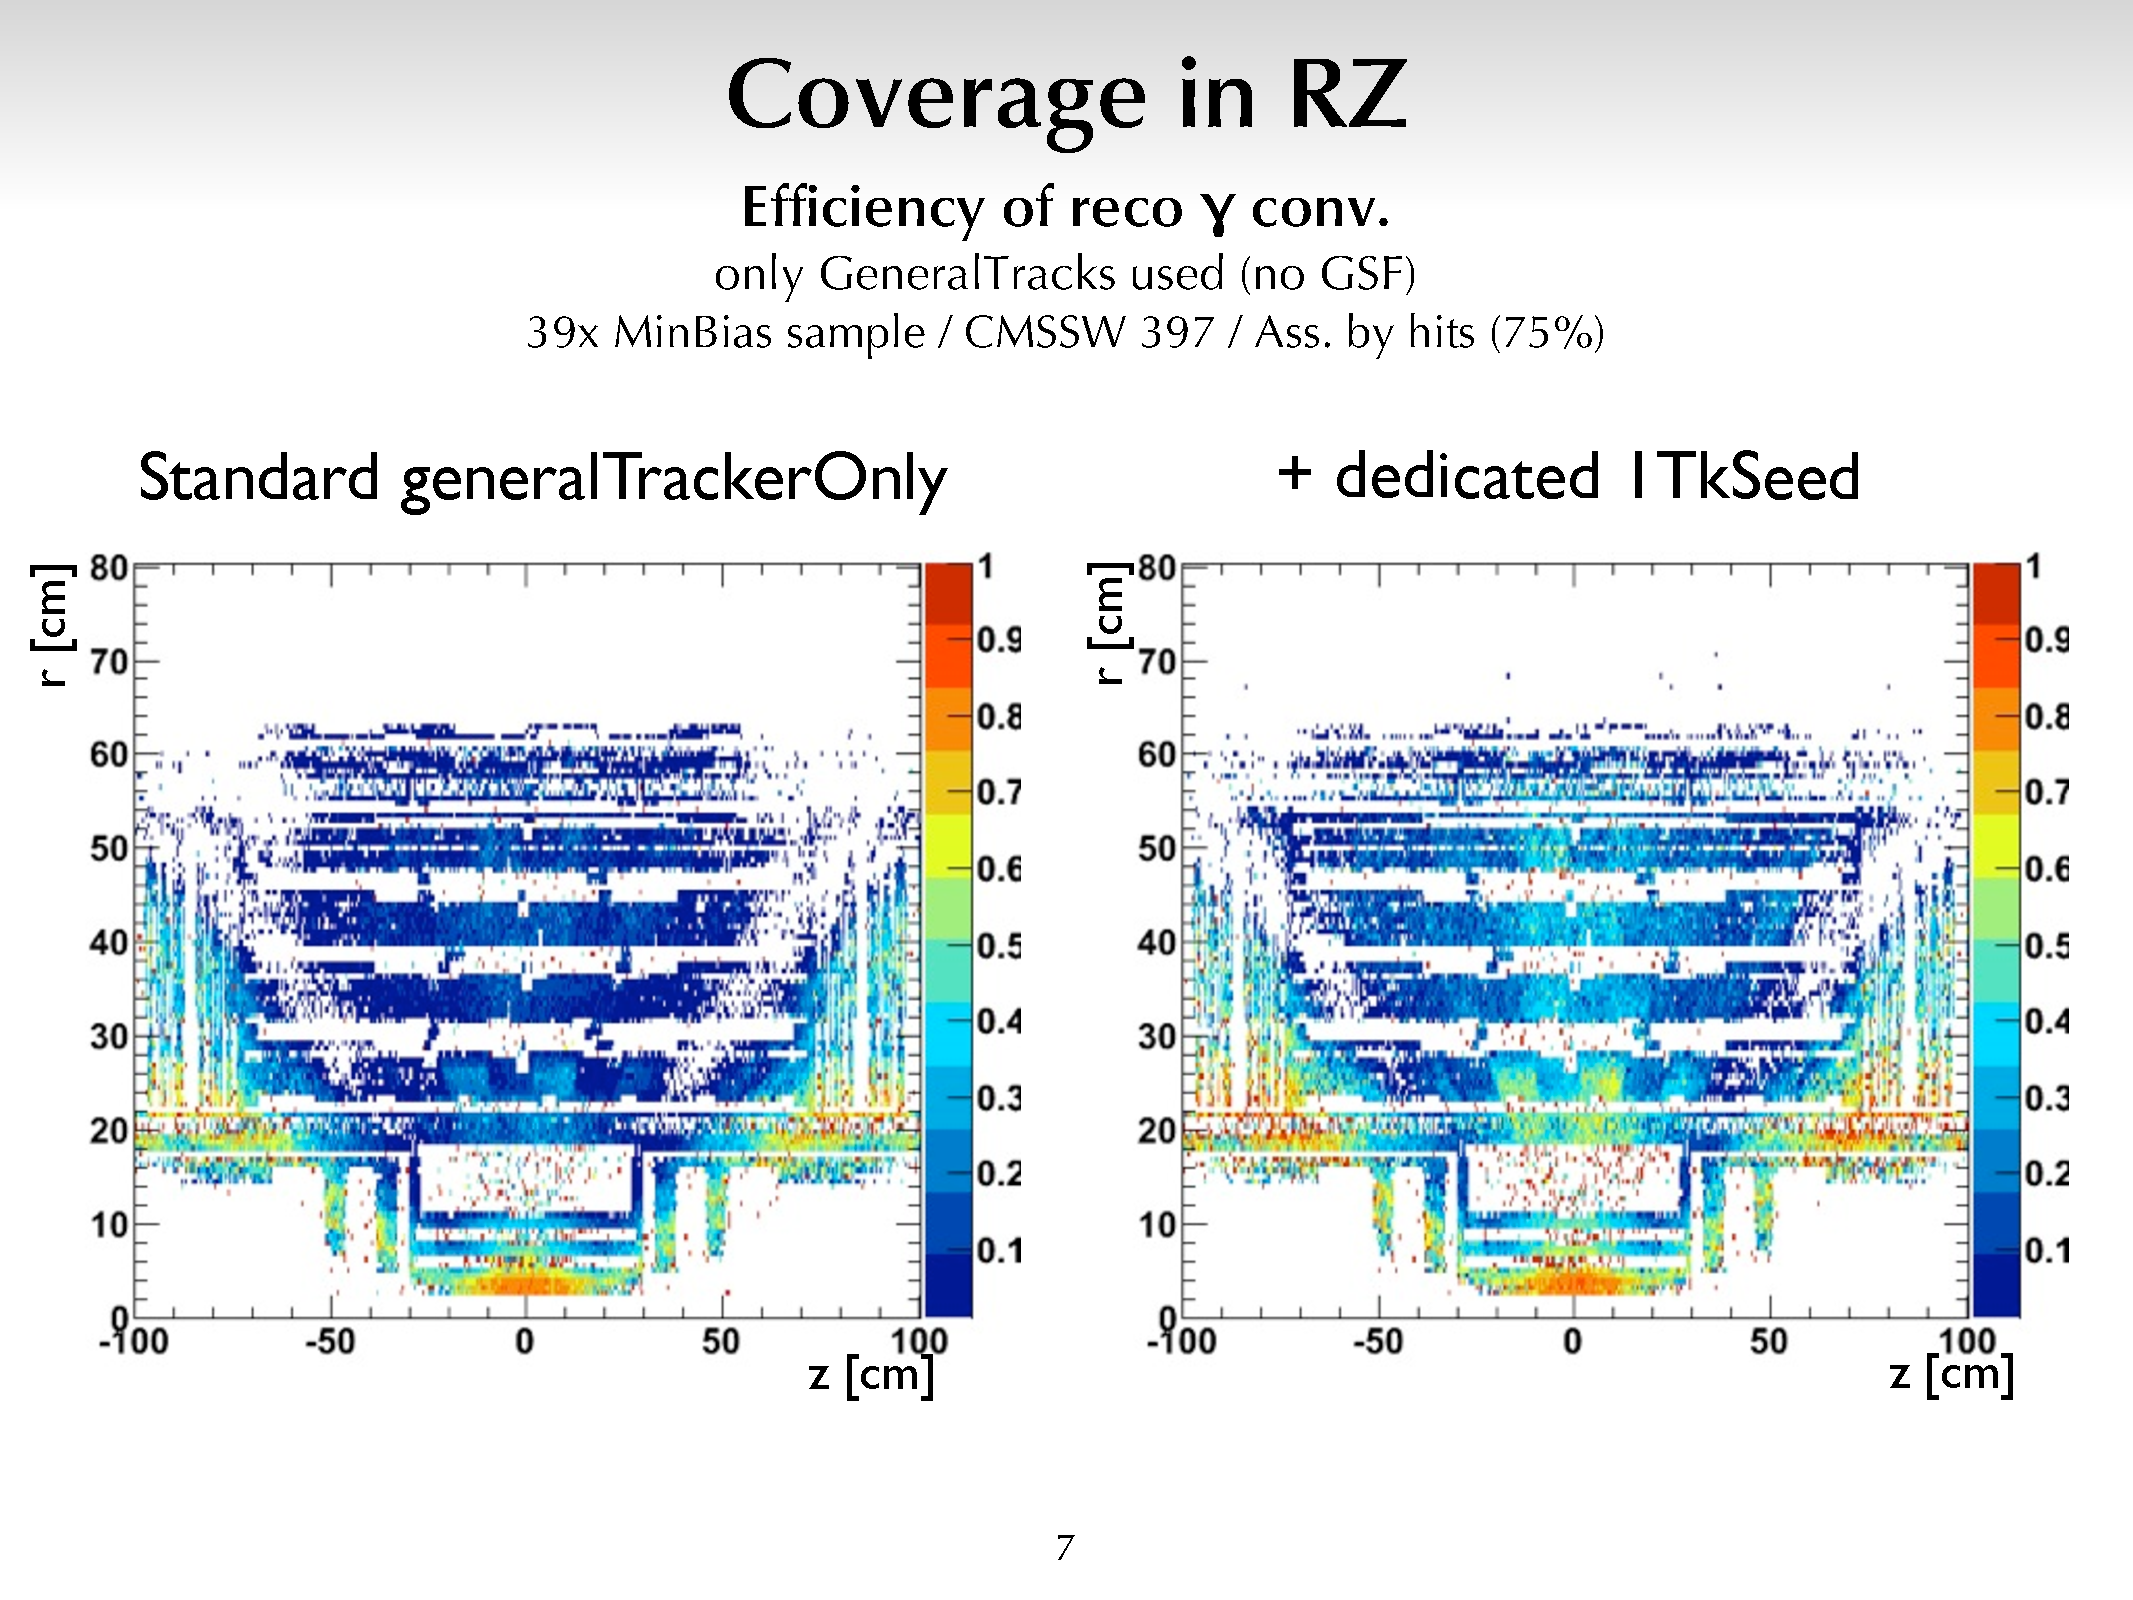
\includegraphics[trim=0cm 3cm 18.5cm 9cm, clip=true,width=.4\textwidth]{fig/singleLegCoverage.pdf}}
\subfigure[]{
\label{subfig:RZCoverageDed}
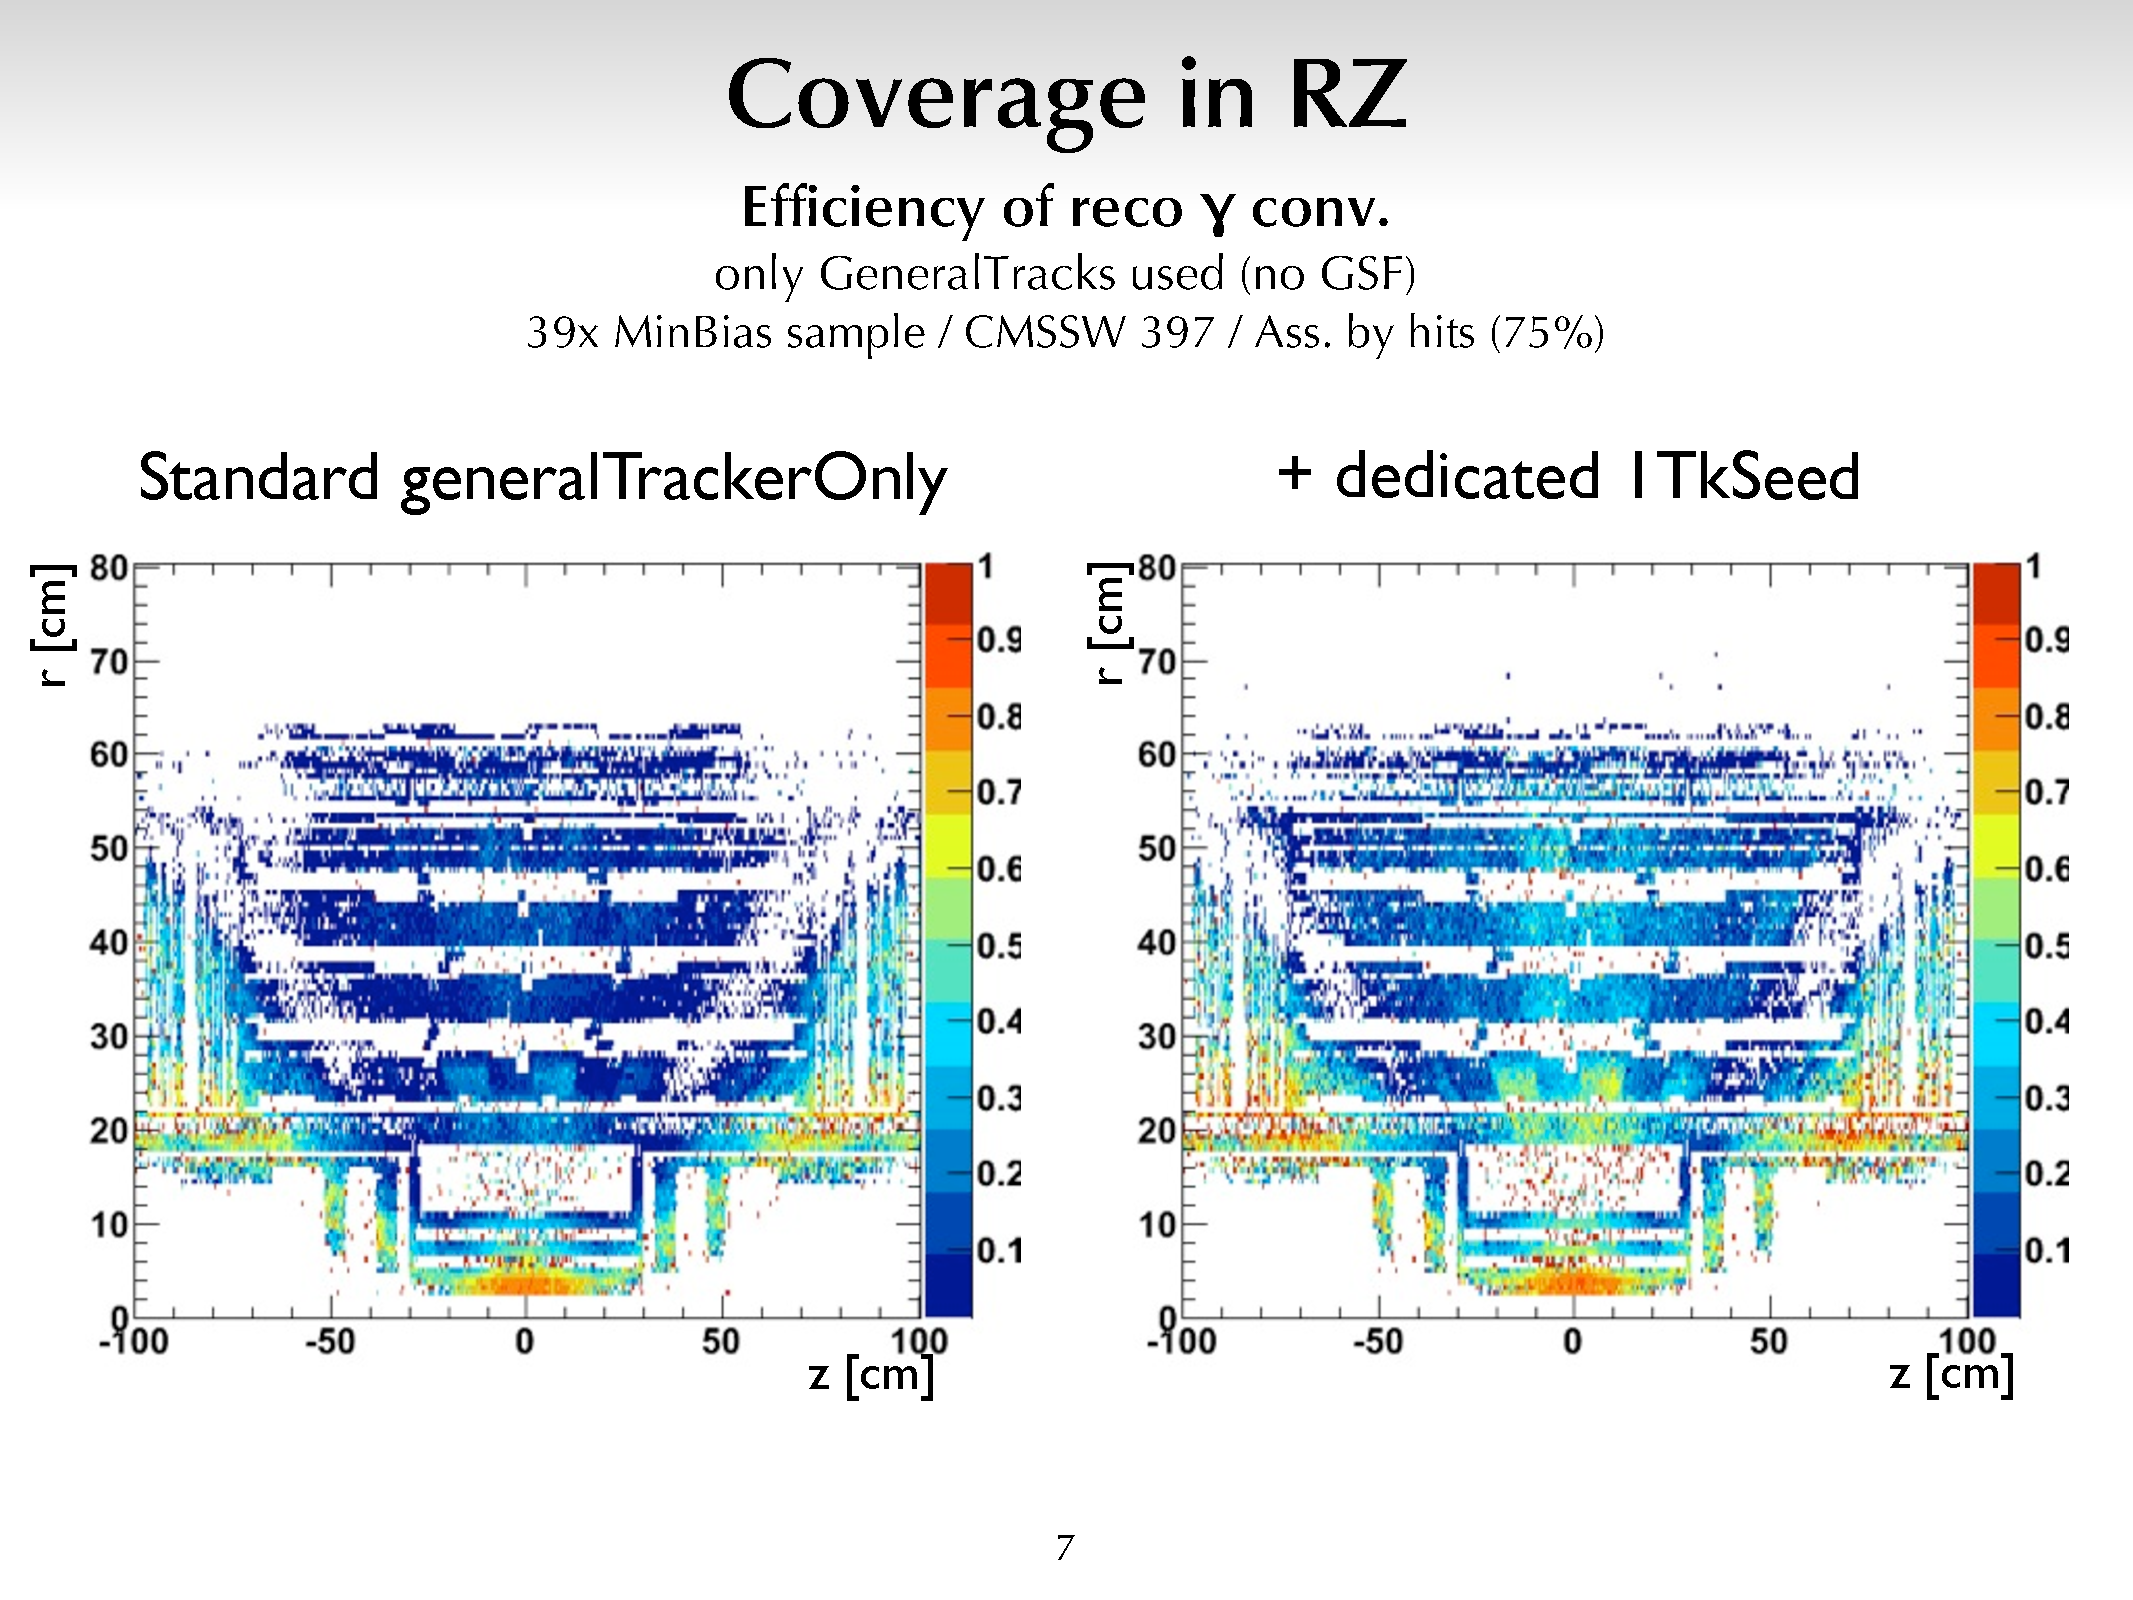
\includegraphics[trim=18.5cm 3cm 0cm 9cm, clip=true,width=.4\textwidth]{fig/singleLegCoverage.pdf}}
\caption{Reconstruction efficiency as a function of the conversion vertex position in the $(z,R)$ plane, evaluated with simulated data using only the standard CMS algorithms~\subref{subfig:RZCoverageStd}  or including the dedicated conversion algorithm~\subref{subfig:RZCoverageDed}. }
\label{fig:RZCoverage}
\end{figure}


In the overall increase of reconstruction efficiency we account also the improved efficiency in the transition region between the Tracker barrel and endcap.  
Figure~\ref{fig:RZCoverage} shows the reconstruction efficiency as a function of the conversion vertex position in the $(z,R)$ plane, evaluated with simulated data using only the standard CMS algorithms (Fig.~\ref{fig:RZCoverage}~\subref{subfig:RZCoverageStd} ) or including our dedicated algorithm (Fig.~\ref{fig:RZCoverage}~\subref{subfig:RZCoverageDed} ). An increase of efficiency is visible in less populated area around $|\eta| \sim 1.2$ when the dedicated algorithm is adopted. This improvement is extremely useful to determine  the amount of material in the transition region as well as to increase the detector acceptance for physics studies.



Figure.~\ref{fig:ptPerf} shows the reconstruction efficiency enhancement due to the  dedicated algorithm as a function of the transverse momentum of the produced lepton tracks. The algorithm contributes to reconstruct mainly the low $\rm p_T$ tracks, whereas the leading track is, by design, reconstructed by the standard algorithms.

\begin{figure}[h]
\centering
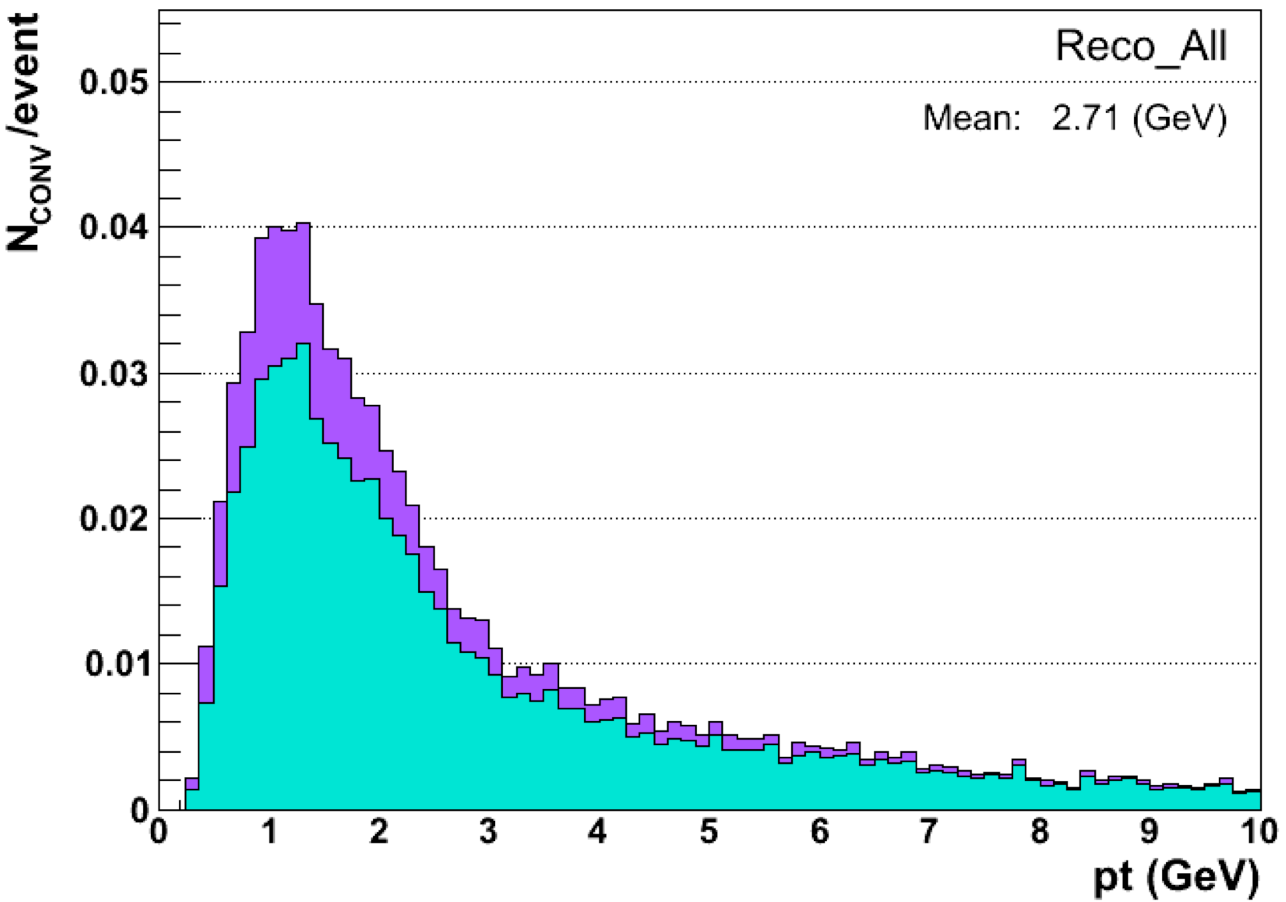
\includegraphics[width=.4\textwidth]{fig/singleLegPt.png}
\caption{Fraction of simulated and reconstructed photon conversions as a function of the transverse momentum of the produced lepton tracks, using only standard tracking algorithms (green) or also the dedicated algorithm (purple). }
\label{fig:ptPerf}
\end{figure}





In terms of processing time per event, this dedicated tracking sequence well fits the available time quota imposed by the reconstruction constraints in the LHC high luminosity  environment.  The good time performance is again a consequence of the demanding requirements applied to limit the number of combinations to examine.
Moreover some of the topological concepts exploited by our algorithm have been adopted also to optimize the processing time of the standard photon conversion reconstruction  in CMS, allowing to gain a factor of 15 in processing time with a smarter preselection of the tracks to be paired~\cite{recoImprovement}. This preselection is built on the same criteria used to identify the expected position of a conversion vertex from a single track. It avoid to pair a track with all the opposite-charge tracks before rejecting it as not compatible with a conversion in the Tracker material.

\section{Conclusions}
\label{section_conclusions}

The photon conversions in the detector material is not just a nuisance in the event reconstruction of HEP experiments, but can be also extremely useful 
We have developed in CMS	a dedicated tracking for photon  conversions that,
exploiting their topology, enhances the reconstruction efficiency by a factor of 20\% to 200\% depending on the radial distance from the beamline.

\section*{References}
\bibliographystyle{unsrt}
\bibliography{biblio}{}

%
%\bibitem{chic}
%{CMS Collaboration},
%\newblock{Observation of the $\chi_c$ states with 1.1 fb$^{-1}$},
%\Journal{CMS Detector Performance Summaries}{CMS-DP-2011-011}{http://cdsweb.cern.ch/record/1369247}{2011}
%
\end{document}
